% NOTE: requires \usepackage{subcaption} in the preamble (in addition to graphicx, tikz, tabularx already used).
% NOTE: For figure/table numbers to be CLICKABLE (jump to the figure/table when clicked),
% the main document preamble must load \usepackage{hyperref} (ideally last, after other packages).
% With hyperref loaded, every \ref{...} / \autoref{...} below automatically becomes a clickable link.

\setcounter{chapter}{10}
\chapter*{Chapter (10): Hardware \& Implementation}
\addcontentsline{toc}{chapter}{Chapter (10): Hardware \& Implementation}
\setcounter{section}{0}

\section{Chapter Preview}
This chapter details the physical integration and mechanical/electrical design of the Sanad prototype. It explains chassis modifications, drivetrain design calculations, PID motor control tuning, power distribution circuits, and concludes with a detailed Bill of Materials (BOM) cost breakdown.

\section{Wheelchair Modifications Over the Manual Platform}
All physical build decisions, from wheelchair frame modifications to the power system, are documented in this chapter in enough detail for replication. This chapter describes the physical implementation of the Sanad smart wheelchair system, including mechanical modifications, motor control architecture, hardware interfacing, and power distribution. The system integrates multiple sensing and interaction modalities while maintaining the structural integrity and safety of the original wheelchair platform.

The original wheelchair platform is a foldable electric wheelchair equipped with two 24\,V, 250\,W brushed DC motors and a 24\,V, 12\,Ah lead-acid battery system capable of carrying up to 120\,kg. This section describes how the base platform was modified to host the sensors, compute units, and assistive modules required for autonomous navigation and human-robot interaction. Figure~\ref{fig:wheelchair-base-views} shows the unmodified base platform before any modifications were carried out.

\begin{figure}[H]
    \centering
    \begin{subfigure}[t]{0.48\textwidth}
        \centering
        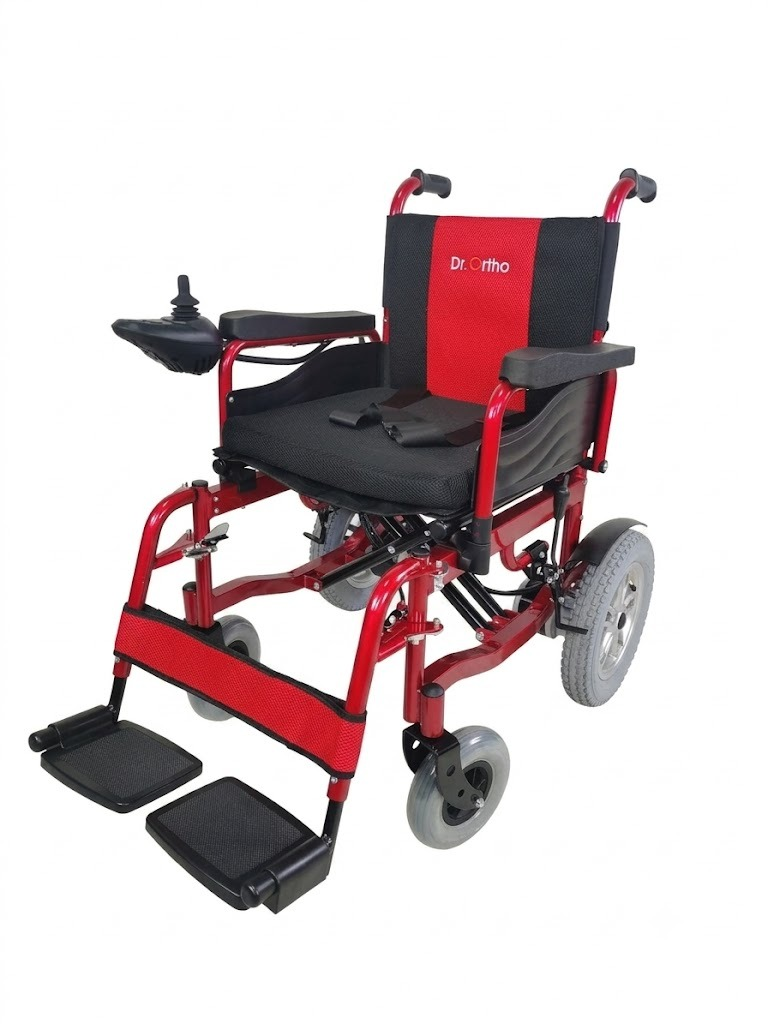
\includegraphics[height=0.32\textheight,keepaspectratio]{figures/ch10/wheelchair-platform}
        \caption{Front view.}
        \label{fig:wheelchair-platform}
    \end{subfigure}\hfill
    \begin{subfigure}[t]{0.48\textwidth}
        \centering
        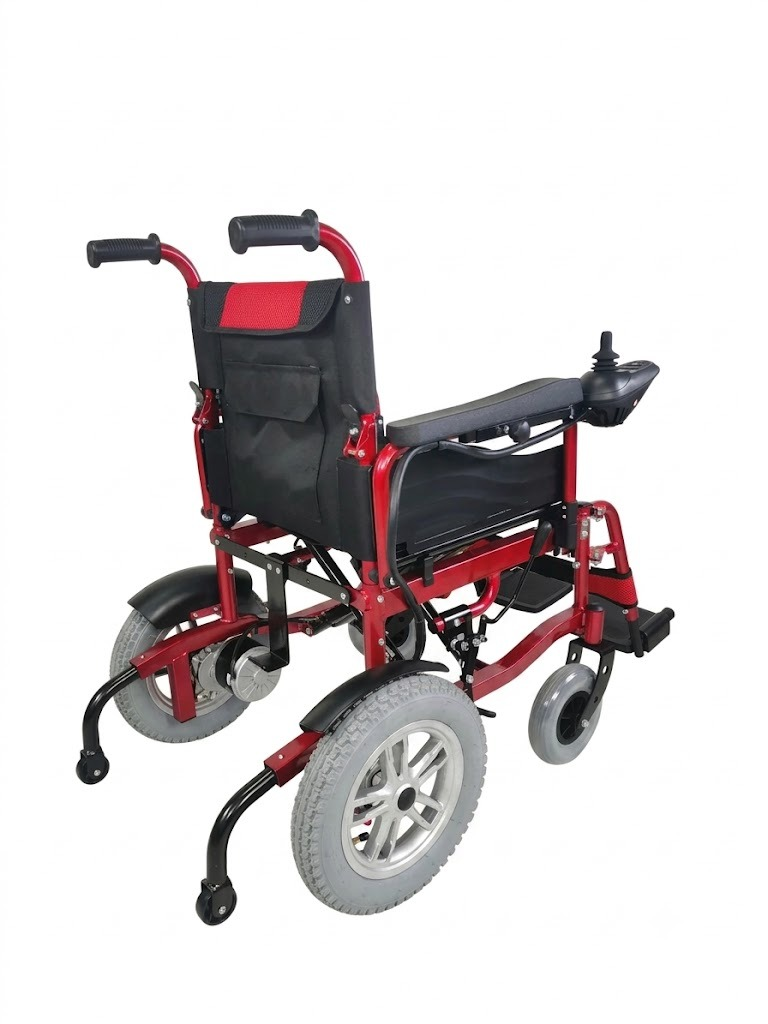
\includegraphics[height=0.32\textheight,keepaspectratio]{figures/ch10/structural-overview}
        \caption{Rear view.}
        \label{fig:structural-overview}
    \end{subfigure}
    \caption{Base wheelchair, real photographs: (a) front view, (b) rear view.}
    \label{fig:wheelchair-base-views}
\end{figure}

\subsection{Base Platform and Mechanical Integration}

To support autonomous navigation, obstacle avoidance, and assistive interaction, a set of sensors and actuators were added to the base wheelchair frame using custom 3D-printed and welded mounts. Each subsystem was positioned to maximize sensor coverage while keeping the wheelchair's footprint, weight distribution, and foldability largely unchanged.

Figure~\ref{fig:structural-overview-diagram} presents a structural overview of all hardware modifications and illustrates how each subsystem interfaces with the Raspberry Pi~5, which serves as the central computing unit of the wheelchair. The subsections that follow walk through how each of these subsystems was physically integrated into the platform, grouped by function: navigation sensing, drivetrain instrumentation, and assistive modules.

\begin{figure}[H]
    \centering
    % Replace the file name with your own image
    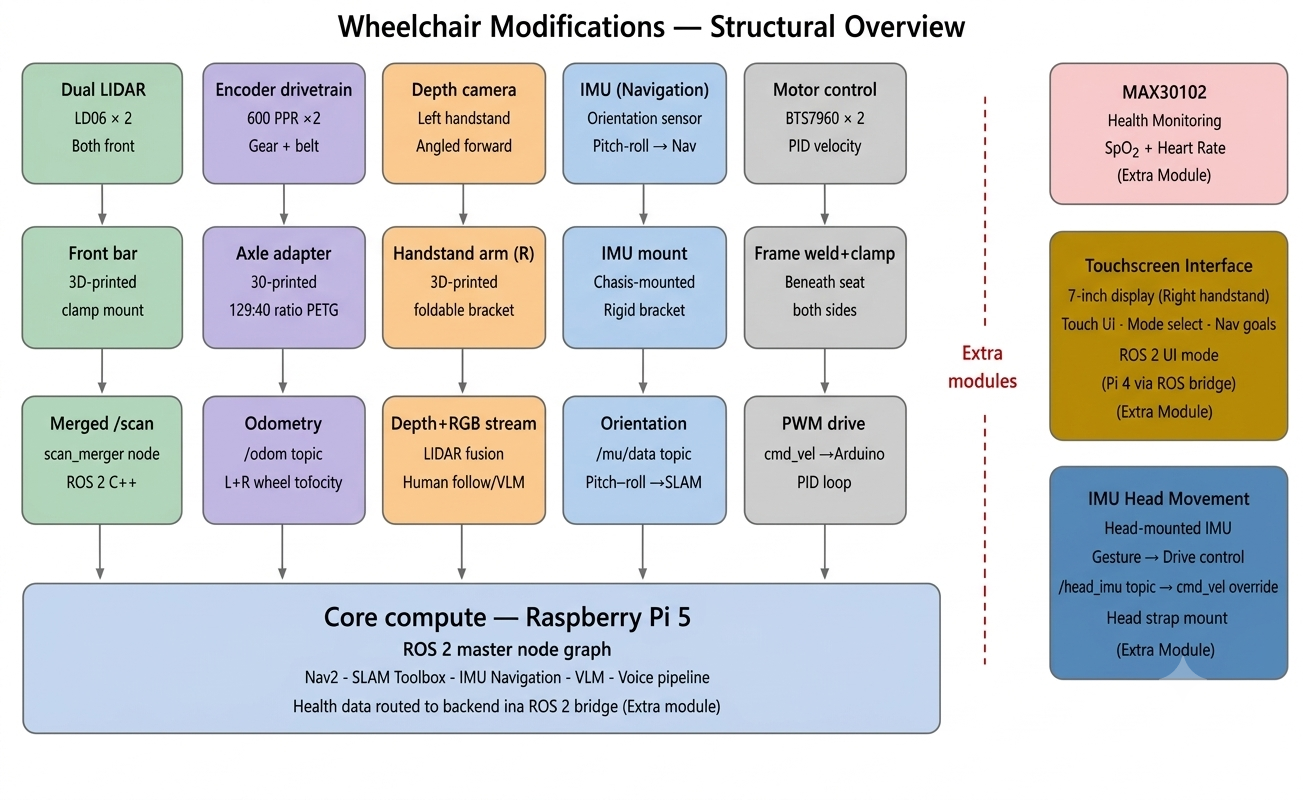
\includegraphics[width=\textwidth]{figures/ch10/structural-overview-diagram}
    \caption{Structural overview of the wheelchair modifications and the data flow .}
    \label{fig:structural-overview-diagram}
\end{figure}

\subsection{Navigation Sensor Integration}

The navigation stack relies on three sensing modalities -- LiDAR, an RGB-D camera, and an IMU -- each mounted so as to give the system consistent, interference-free coverage of the environment ahead of and around the wheelchair.

\subsection*{Dual LiDAR Mount}
Two LD06 LiDAR sensors were mounted at the front of the wheelchair using a custom 3D-printed front bar.
\begin{itemize}
\item It provides the environmental information required for mapping and localization.
\item It enables accurate obstacle detection and safe navigation.
\item It improves the reliability of autonomous navigation.
\end{itemize}

% TODO (pending clarification): user asked to check whether this figure has a lot of
% empty space below it, and if so, to merge the LiDAR holder figure's (a) and (b)
% subfigures into it instead of keeping them as a separate two-part figure below.
% Not applied yet -- waiting to confirm this is the intended figure pair.
Figure~\ref{fig:lidar-mount} shows the LD06 LiDAR sensor mounted at the front of the wheelchair using the custom 3D-printed bar described above.

\begin{figure}[H]
    \centering
    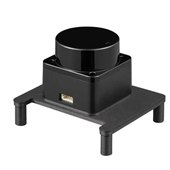
\includegraphics[height=0.22\textheight,keepaspectratio]{figures/ch10/lidar-mount}
    \caption{LD06 LiDAR sensor mount at the front of the wheelchair.}
    \label{fig:lidar-mount}
\end{figure}

Figure~\ref{fig:lidar-holder} shows the CAD model of the LiDAR holder alongside the corresponding fabricated 3D-printed part used to secure each sensor.

\begin{figure}[H]
    \centering
    \begin{subfigure}[t]{0.48\textwidth}
        \centering
        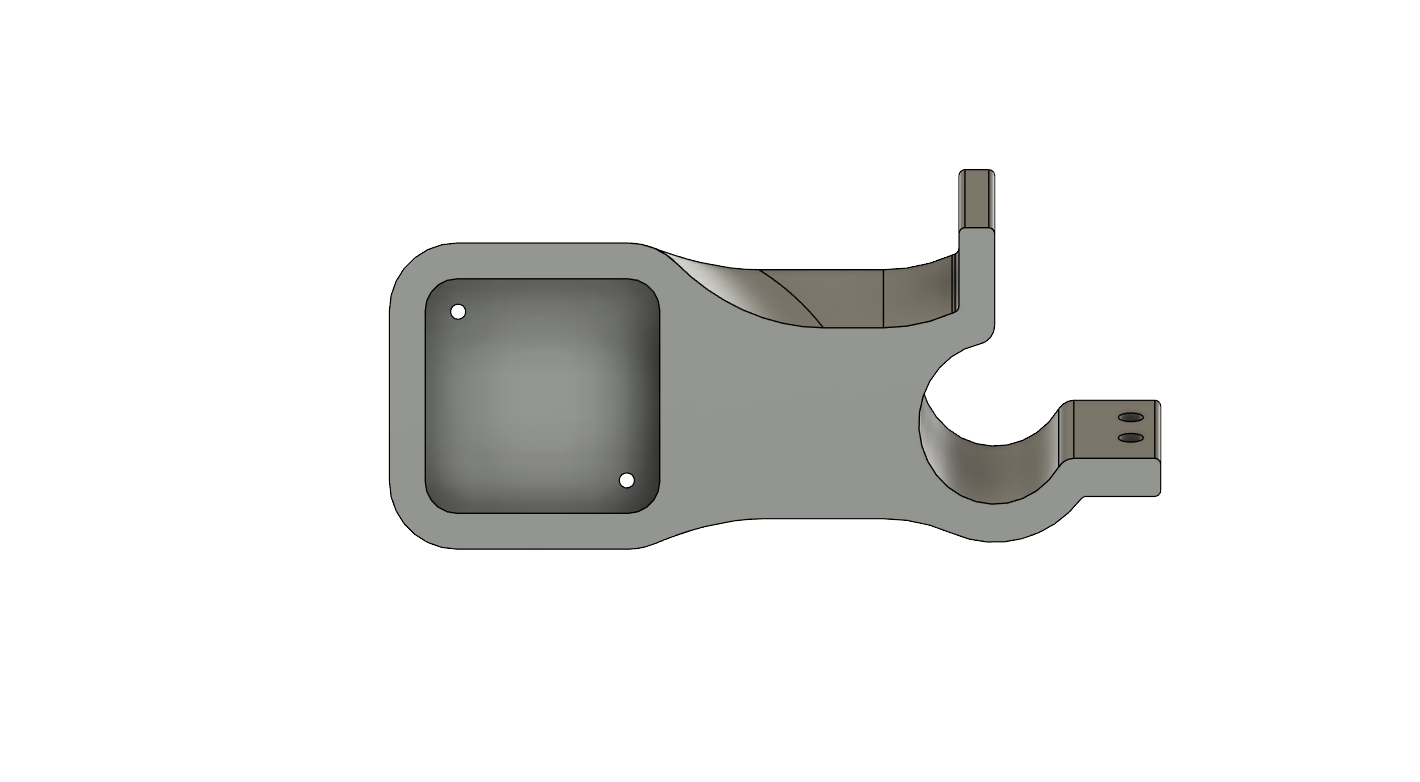
\includegraphics[height=0.22\textheight,keepaspectratio]{figures/ch10/lidar-holder-cad}
        \caption{3D CAD model (Autodesk Fusion).}
        \label{fig:lidar-holder-cad}
    \end{subfigure}\hfill
    \begin{subfigure}[t]{0.48\textwidth}
        \centering
        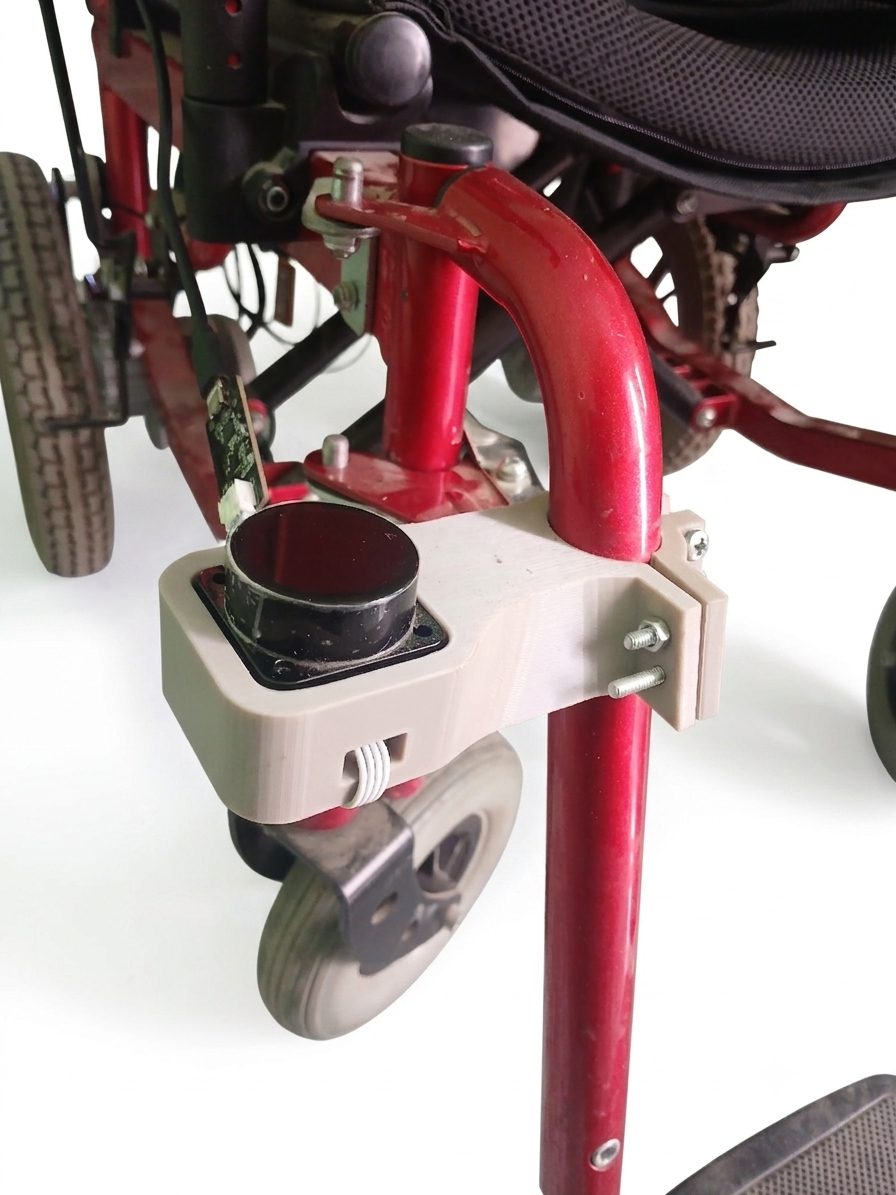
\includegraphics[height=0.22\textheight,keepaspectratio]{figures/ch10/lidar-holder-real}
        \caption{3D-printed part after fabrication.}
        \label{fig:lidar-holder-real}
    \end{subfigure}
    \caption{LiDAR holder: (a) 3D CAD model, (b) fabricated 3D-printed part.}
    \label{fig:lidar-holder}
\end{figure}

The front dual-LiDAR bar shown in Figure~\ref{fig:lidar-holder} fixes both LD06 units at a fixed relative angle, guaranteeing the combined field of view assumed in the SLAM configuration.

\subsection*{Depth Camera Mount}
The RGB-D camera was installed on the left armrest using an angled bracket, oriented forward and slightly downward so that it can track people and obstacles directly ahead of the wheelchair.
\begin{itemize}
\item Human following.
\item Object detection.
\item Environment perception.
\end{itemize}

Figure~\ref{fig:depth-camera-mount} shows the RGB-D camera mounted on the left armrest in this forward-and-downward-facing orientation.

\begin{figure}[H]
    \centering
    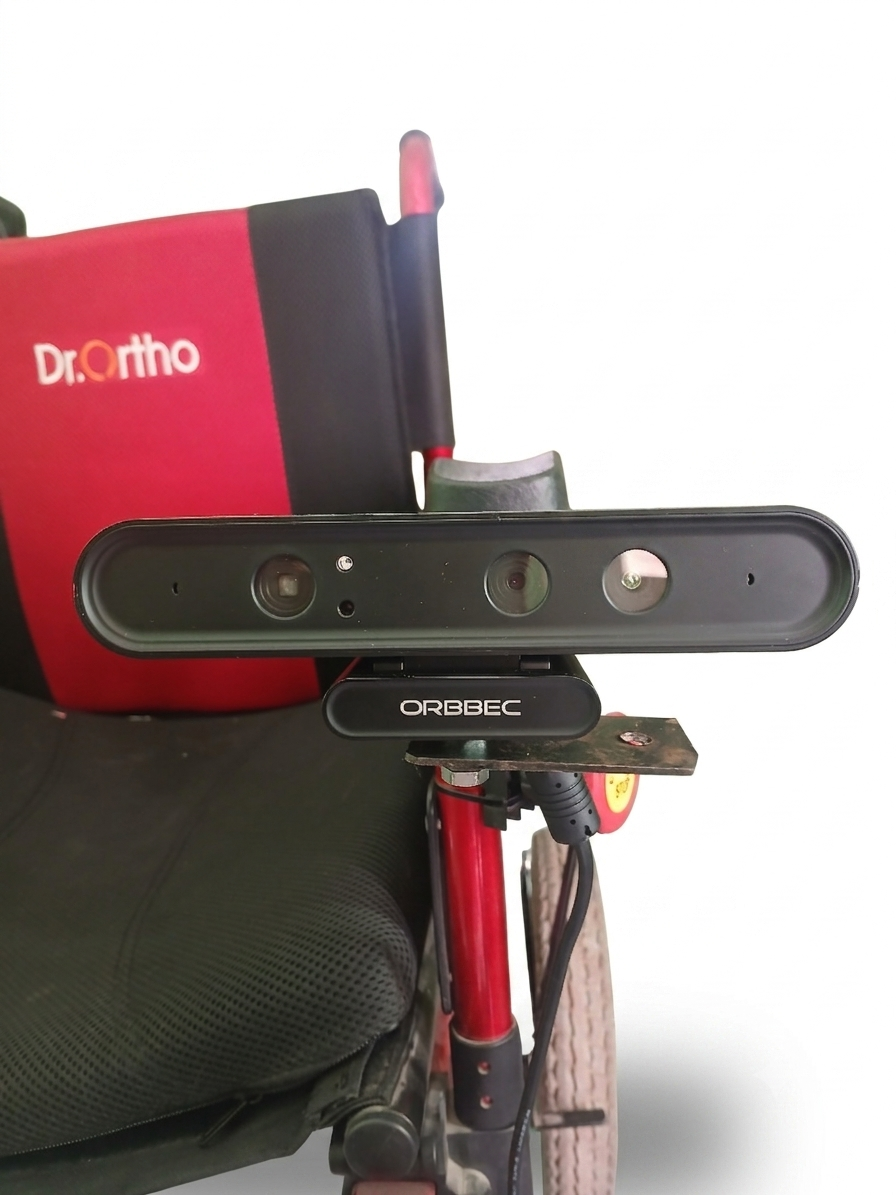
\includegraphics[height=0.18\textheight,keepaspectratio]{figures/ch10/depth-camera-mount}
    \caption{RGB-D camera mount on the left armrest.}
    \label{fig:depth-camera-mount}
\end{figure}

\subsection*{Navigation IMU Mount}
An inertial measurement unit (IMU) was rigidly mounted to the chassis beneath the seat to provide continuous orientation data for the navigation stack. Working alongside the LiDAR and depth camera, this sensor improves the robustness of SLAM-based localization, particularly when the wheelchair encounters uneven surfaces or slight inclines.
\begin{itemize}
\item Measures the wheelchair orientation.
\item Improves localization accuracy and overall navigation performance.
\end{itemize}

Figure~\ref{fig:imu-mount} shows the IMU rigidly mounted beneath the wheelchair seat.

\begin{figure}[H]
    \centering
    \tikz[baseline=(img.base)] \node[inner sep=0pt,fill=white] (img) {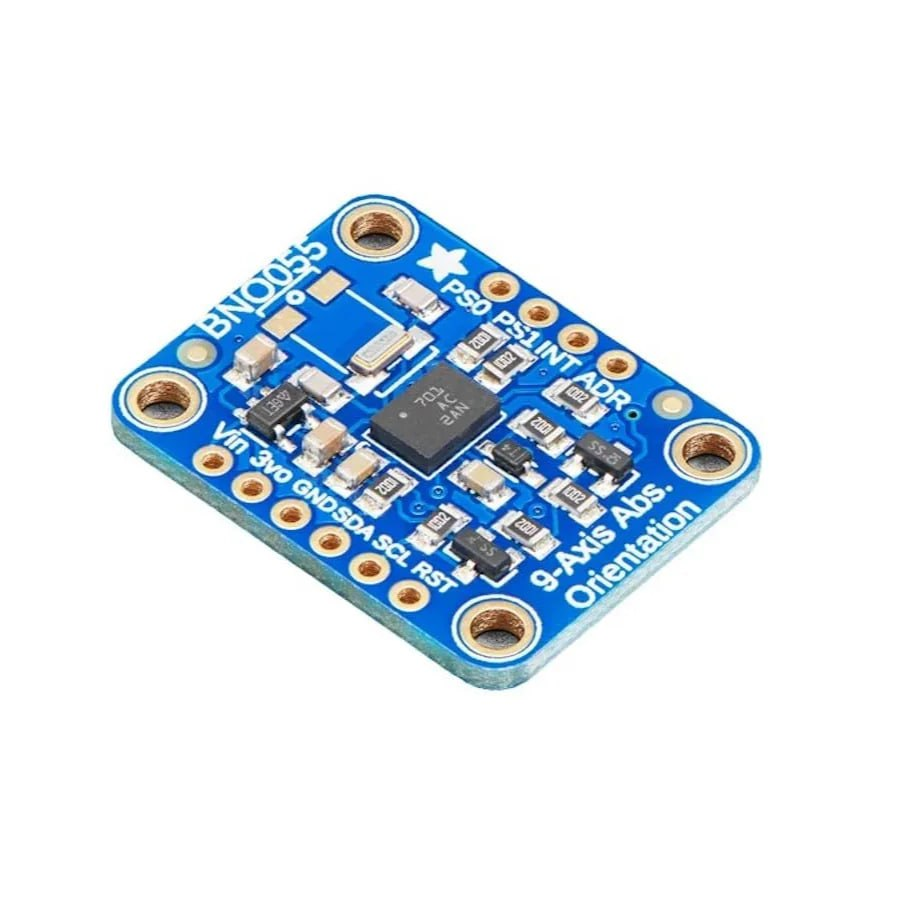
\includegraphics[height=0.18\textheight,keepaspectratio]{figures/ch10/imu-mount}};
    \caption{IMU mounted beneath the wheelchair seat.}
    \label{fig:imu-mount}
\end{figure}

\subsection{Drive System Integration}

Closed-loop control of the drivetrain requires accurate wheel-speed feedback and current-capable motor drivers, both integrated close to the wheels to keep cabling short and signal quality high.

\subsection*{Encoder Installation}
To close the velocity control loop and support accurate odometry, an incremental rotary encoder was mechanically coupled to each drive wheel through a custom GT2 belt-and-pulley transmission. The encoder output is read by the Arduino Nano and used both for real-time speed control and for generating odometry data for the ROS 2 navigation stack.
\begin{itemize}
\item Measure wheel speed accurately.
\item Provide feedback for the PID speed controller.
\item Generate odometry information for localization and navigation.
\item Maintain stable motor speed under varying loads and terrain conditions.
\item Improve motion accuracy during autonomous navigation.
\end{itemize}

Additional encoder-based odometry is also used to detect slip and improve the stability of closed-loop velocity control across variable loads, ensuring the wheelchair follows commanded paths with minimal drift. Figure~\ref{fig:encoder-drivetrain} shows the incremental rotary encoder module used for this purpose.

% TODO (pending clarification): same possible candidate as the LiDAR figures above --
% if this is the figure with a lot of empty space below it, the encoder holder
% figure's (a) and (b) subfigures could be merged into it instead. Not applied yet.
\begin{figure}[H]
    \centering
    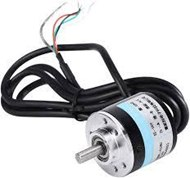
\includegraphics[height=0.18\textheight,keepaspectratio]{figures/ch10/encoder-drivetrain}
    \caption{Incremental rotary encoder module used for wheel speed measurement.}
    \label{fig:encoder-drivetrain}
\end{figure}

\begin{figure}[H]
    \centering
    \begin{subfigure}[t]{0.48\textwidth}
        \centering
        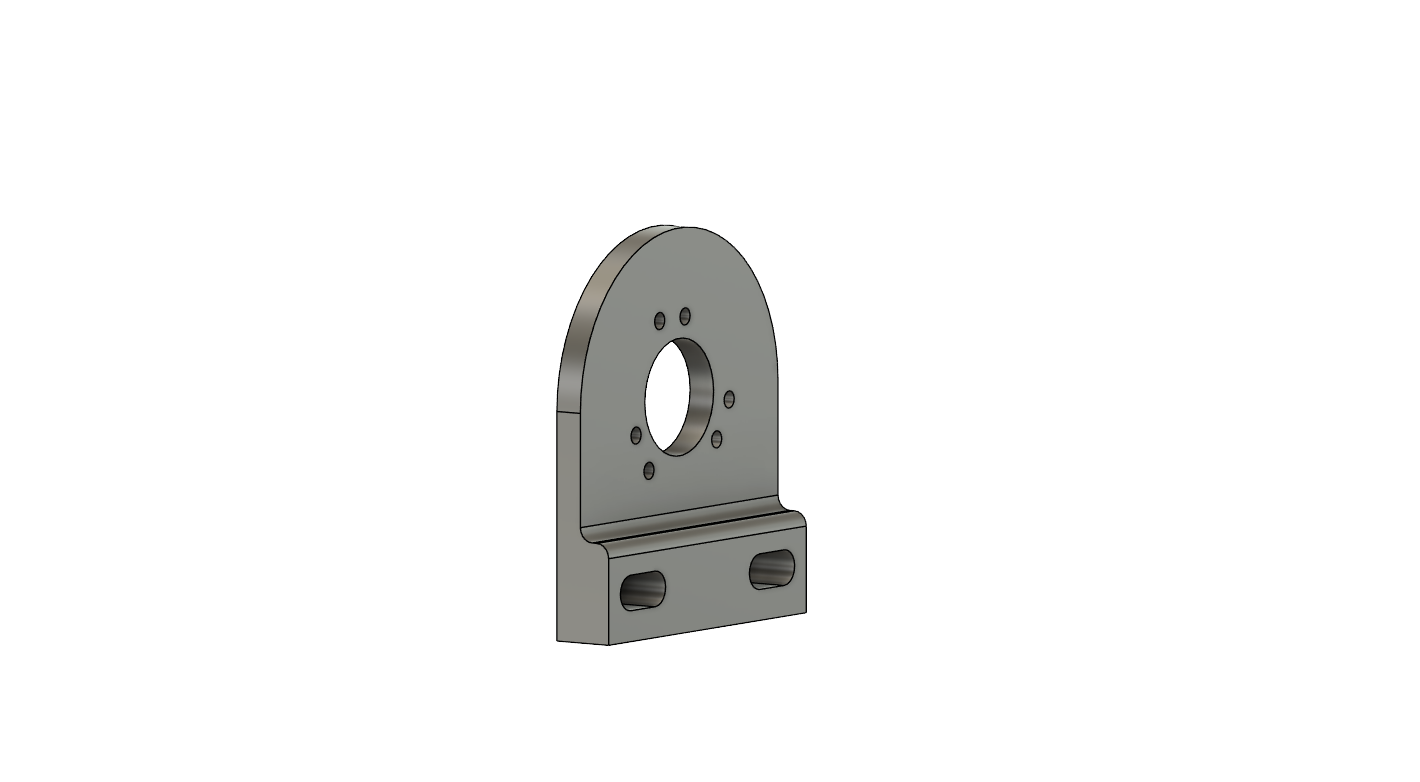
\includegraphics[height=0.22\textheight,keepaspectratio]{figures/ch10/encoder-holder-cad}
        \caption{3D CAD model (Autodesk Fusion).}
        \label{fig:encoder-holder-cad}
    \end{subfigure}\hfill
    \begin{subfigure}[t]{0.48\textwidth}
        \centering
        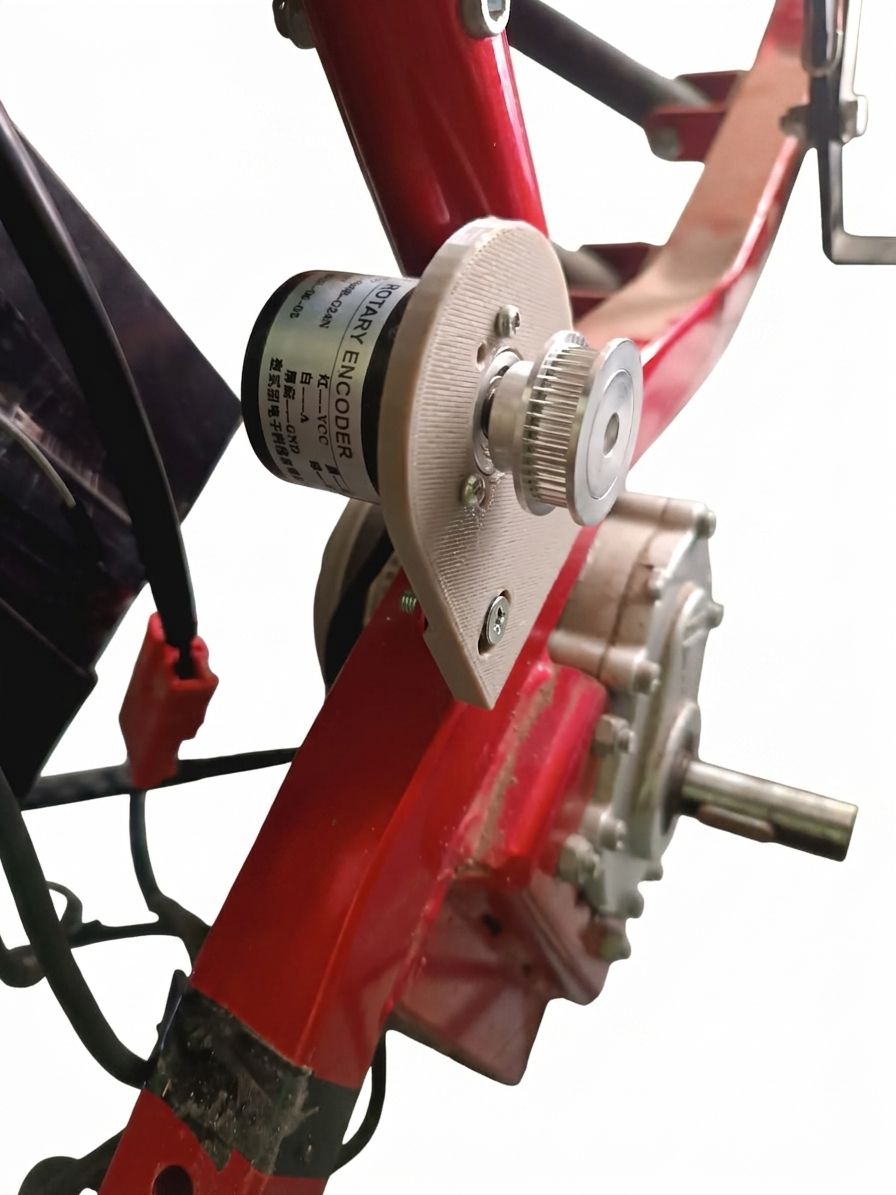
\includegraphics[height=0.22\textheight,keepaspectratio]{figures/ch10/encoder-holder-real}
        \caption{Printed part installed on the chassis.}
        \label{fig:encoder-holder-real}
    \end{subfigure}
    \caption{Encoder holder: (a) 3D CAD model, (b) printed part installed on the chassis.}
    \label{fig:encoder-holder}
\end{figure}

The bracket shown in Figure~\ref{fig:encoder-holder} holds the encoder shaft parallel to the wheel axle so the GT2 belt runs flat with no lateral misalignment.



\subsection*{GT2 Transmission}
To improve wheel speed measurement accuracy and odometry estimation, the wheel encoders were not mounted directly on the motor shafts. Instead, a mechanical transmission system based on a GT2 timing belt and two pulleys was designed to connect the motor shaft to the encoder.

The transmission system consists of:
\begin{itemize}
\item A 129-tooth GT2 pulley mounted on the wheelchair wheel shaft.
\item A 40-tooth GT2 pulley mounted on the encoder shaft.
\item A GT2 timing belt connecting both pulleys.
\end{itemize}

\begin{figure}[H]
    \centering
    \begin{subfigure}[t]{0.48\textwidth}
        \centering
        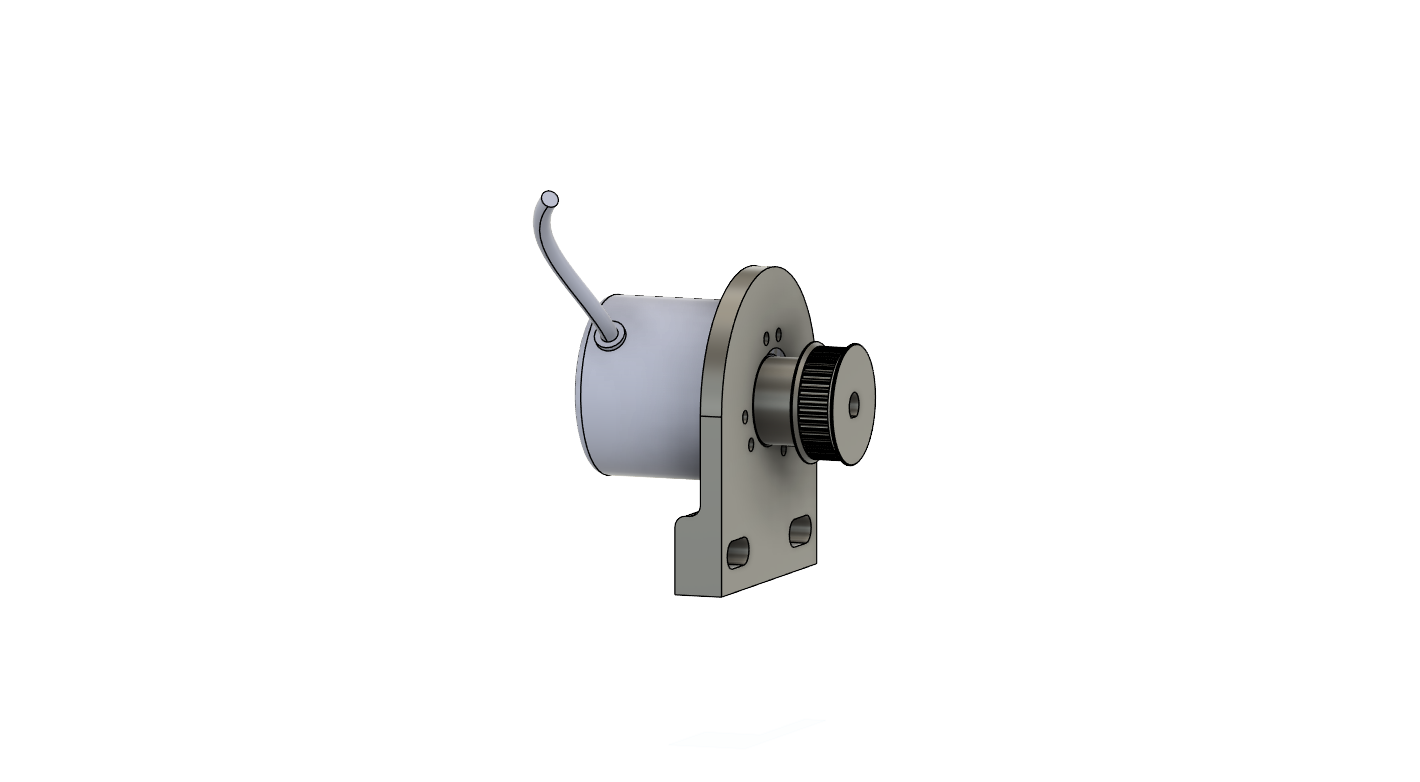
\includegraphics[height=0.20\textheight,keepaspectratio]{figures/ch10/gt2-transmission-cad-assembly}
        \caption{40-tooth GT2 pulley mounted on the encoder shaft.}
        \label{fig:gt2-transmission-cad-assembly}
    \end{subfigure}
    \hfill
    \begin{subfigure}[t]{0.48\textwidth}
        \centering
        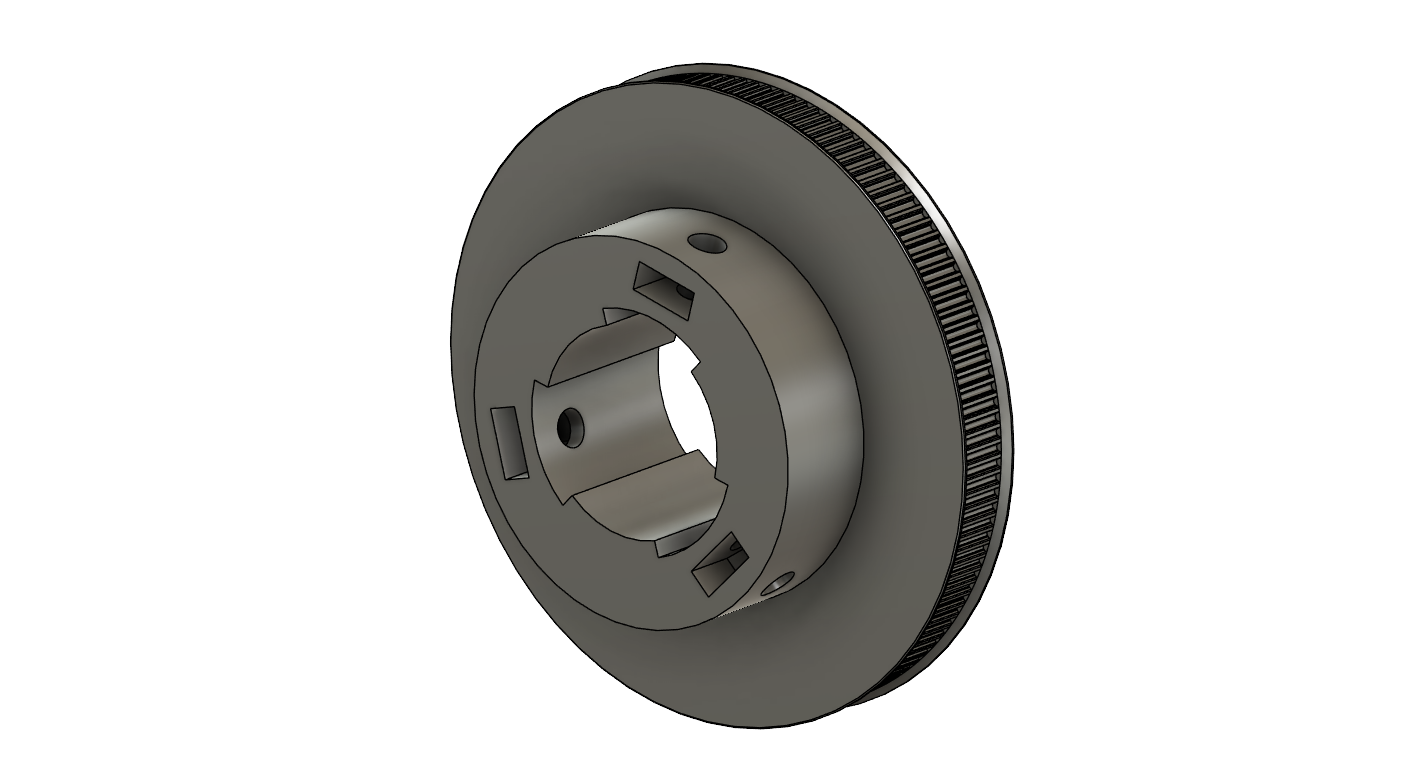
\includegraphics[height=0.20\textheight,keepaspectratio]{figures/ch10/gt2-transmission-real}
        \caption{129-tooth GT2 pulley mounted on the wheel shaft.}
        \label{fig:gt2-transmission-real}
    \end{subfigure}

    \vspace{0.6cm}

    \begin{subfigure}[t]{0.65\textwidth}
        \centering
        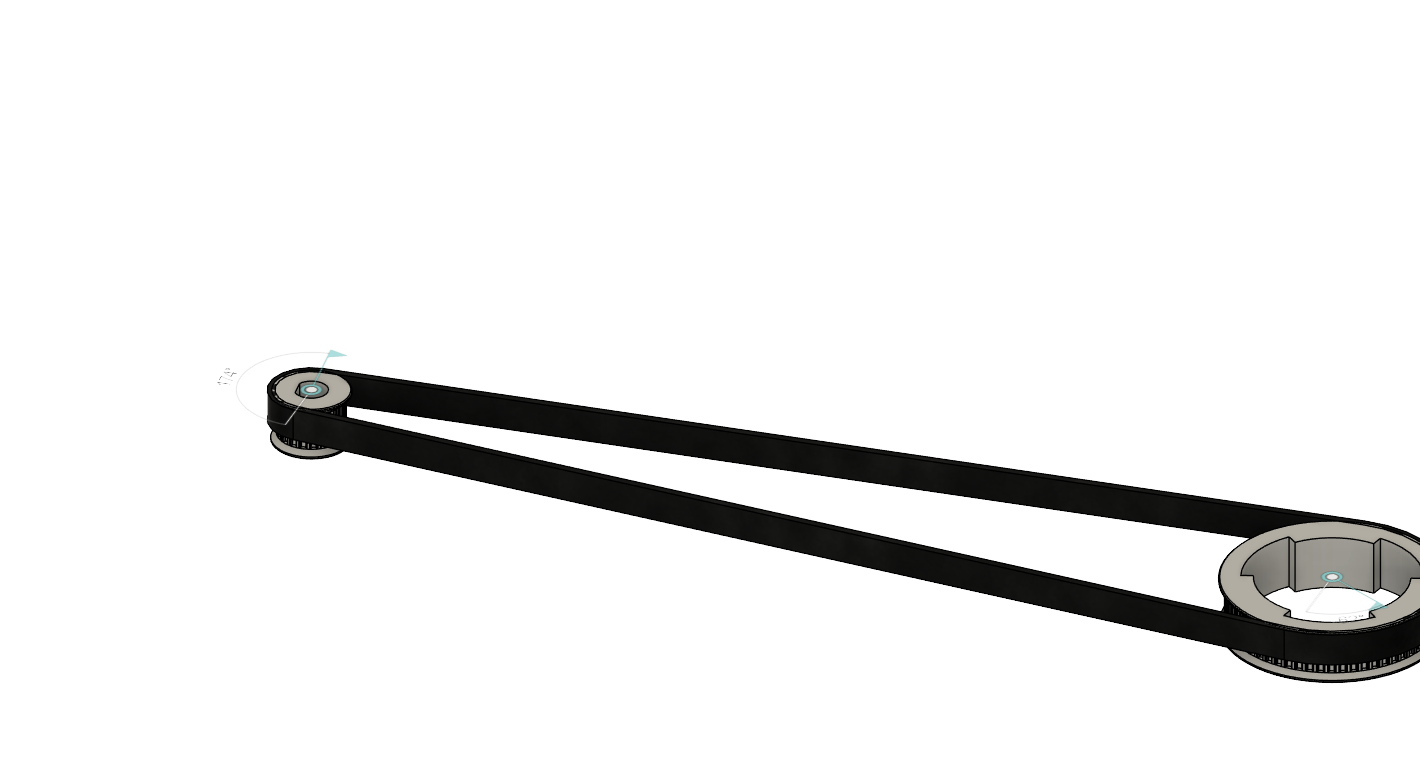
\includegraphics[height=0.20\textheight,keepaspectratio]{figures/ch10/gt2-transmission-cad-exploded}
        \caption{Assembly view showing the 129T and 40T pulleys connected by the belt.}
        \label{fig:gt2-transmission-cad-exploded}
    \end{subfigure}
    \caption{GT2 pulley--belt transmission, CAD models: (a) 40-tooth pulley on the encoder shaft, (b) 129-tooth pulley on the wheel shaft, (c) assembled transmission showing both pulleys connected by the belt.}
    \label{fig:gt2-transmission}
\end{figure}
The 3.225:1 ratio between the 129-tooth and 40-tooth pulleys shown in Figure~\ref{fig:gt2-transmission} is easier to verify visually when each pulley is inspected on its own before seeing both connected by the belt, as in the assembly view above.

The transmission ratio is calculated as:
\[
\text{Gear Ratio} = \frac{129}{40} = 3.225
\]
This means that for every complete revolution of the wheelchair wheel, the encoder rotates approximately 3.225 revolutions. Since the encoder provides 600 pulses per revolution, the effective wheel resolution becomes:
\[
\text{Effective Resolution} = 600 \times \frac{129}{40} = 1935\ \text{pulses per wheel revolution}
\]
Advantages of the GT2 belt transmission:
\begin{itemize}
\item Increases encoder measurement resolution.
\item Improves wheel velocity estimation accuracy.
\item Enhances odometry precision for SLAM and localization.
\end{itemize}
The use of a GT2 timing belt transmission allows the encoder to operate at a higher rotational
speed than the wheel, effectively multiplying the encoder resolution by a factor of 3.225. This
significantly improves the performance of the PID speed controller and the accuracy of wheel
odometry, both of which are critical for reliable autonomous navigation of the smart wheelchair.

\subsection*{Motor Driver Installation}
Two BTS7960 motor drivers were mounted beneath the wheelchair seat, close to the motors, to minimize cable length and voltage drop. Each driver independently controls one of the two 24 V, 250 W brushed DC motors, enabling differential drive and precise speed regulation of the left and right wheels. The drivers receive PWM and direction signals from the Arduino Nano, which executes the motor control algorithm and processes the encoder feedback. Figure~\ref{fig:motor-driver} shows the motor driver board installed beneath the seat.

\begin{figure}[H]
    \centering
    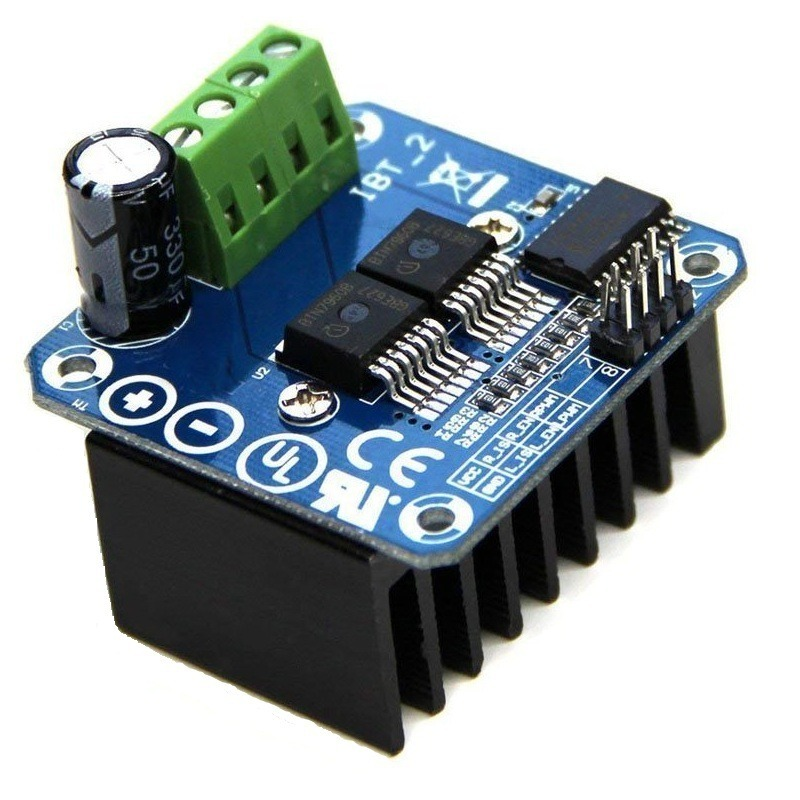
\includegraphics[height=0.18\textheight,keepaspectratio]{figures/ch10/motor-driver}
    \caption{Motor driver board installed under the wheelchair seat.}
    \label{fig:motor-driver}
\end{figure} 
\subsection{Assistive Module Integration}

In addition to the core navigation and mobility subsystems, several modular assistive devices were integrated into the Sanad smart wheelchair to enhance accessibility, usability, and healthcare support. These modules were designed using a plug-and-play architecture, allowing them to be added, removed, or upgraded independently without affecting the operation of the main wheelchair system.

The modular approach provides flexibility to adapt the wheelchair to the specific needs of different users. Depending on the user's physical condition and requirements, assistive modules such as head-motion control, touchscreen interaction, and biometric health monitoring can be enabled or disabled as needed.

\subsection*{Head-Motion Control Unit}
A wearable IMU module was mounted on a head strap, allowing users with limited hand mobility to control the wheelchair through head movements. The sensor continuously measures the orientation and angular motion of the user's head and converts these measurements into navigation commands such as forward motion, turning left, turning right, and stopping. This hands-free control approach provides an alternative interaction method for users who may be unable to operate conventional joysticks or touch interfaces due to physical impairments. The head-mounted configuration ensures stable sensor positioning relative to the user's head, improving measurement accuracy and reducing motion artifacts caused by body movements. Figure~\ref{fig:head-control-unit} shows the wearable IMU head control module.

% TODO (pending clarification): another possible candidate for the "space below /
% merge the a-b figure into it" request. Not applied yet.
\begin{figure}[H]
    \centering
    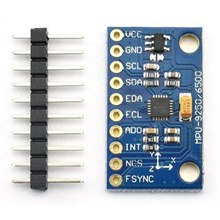
\includegraphics[height=0.18\textheight,keepaspectratio]{figures/ch10/head-control-unit}
    \caption{Wearable IMU head control module.}
    \label{fig:head-control-unit}
\end{figure}

\begin{figure}[H]
    \centering
    \begin{subfigure}[t]{0.48\textwidth}
        \centering
        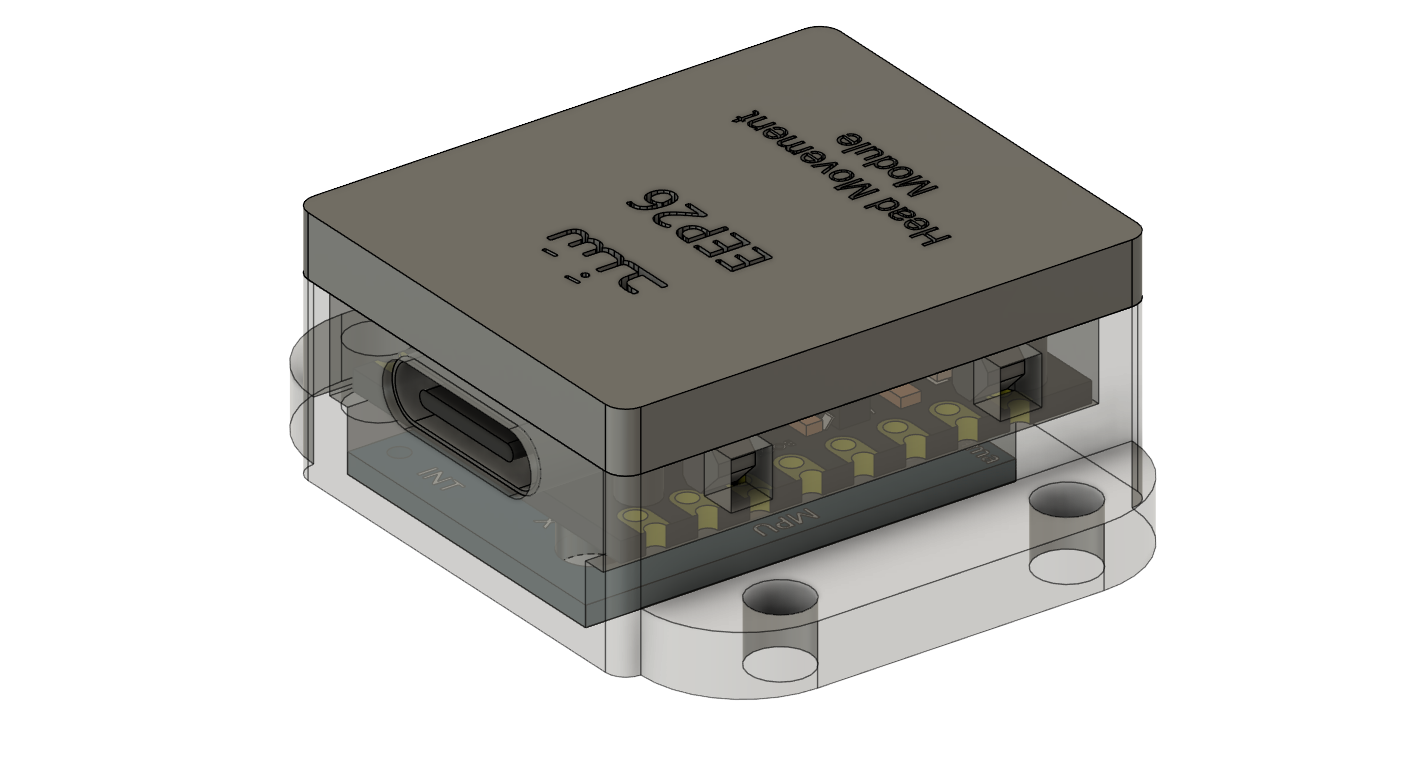
\includegraphics[height=0.20\textheight,keepaspectratio]{figures/ch10/head-unit-cad-front}
        \caption{CAD front view of the shell.}
        \label{fig:head-unit-cad-front}
    \end{subfigure}\hfill
    \begin{subfigure}[t]{0.48\textwidth}
        \centering
        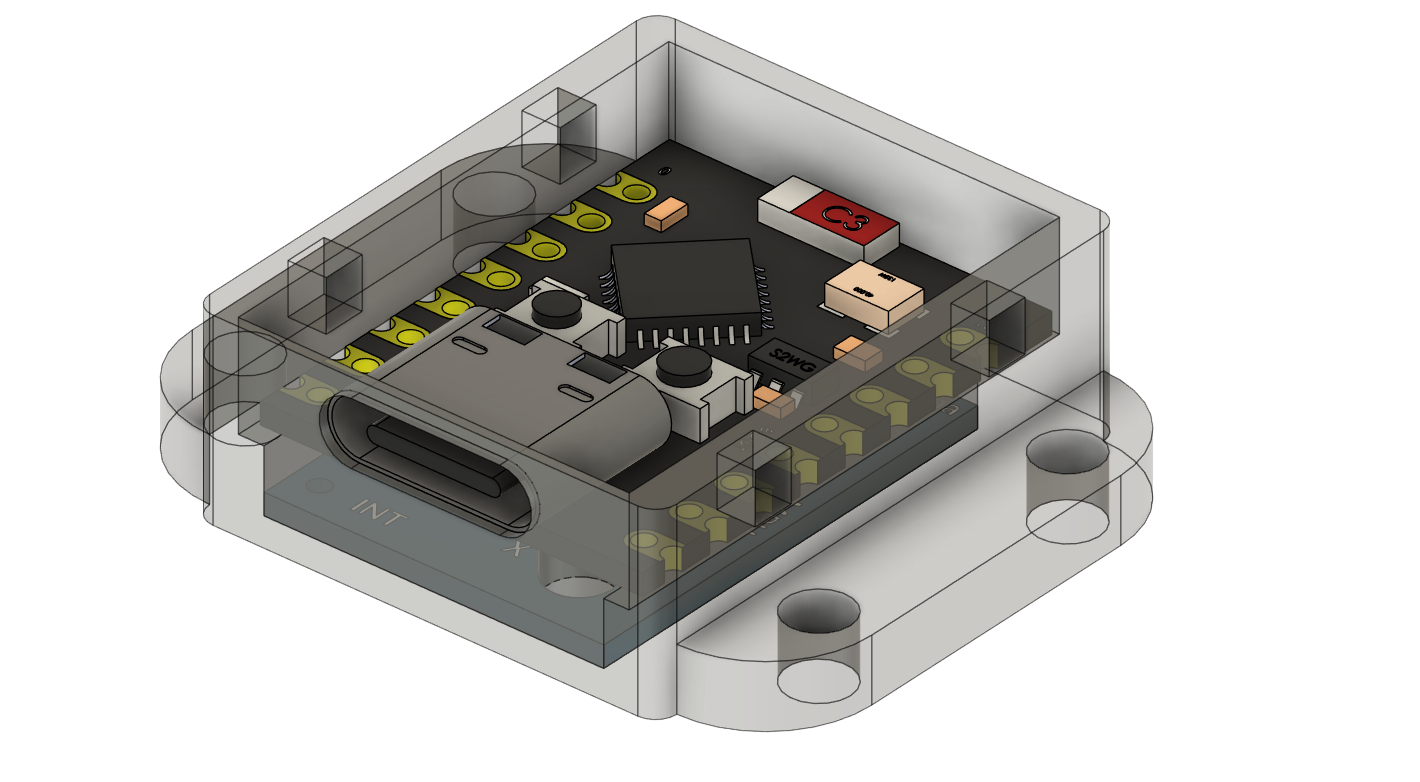
\includegraphics[height=0.20\textheight,keepaspectratio]{figures/ch10/head-unit-cad-internal}
        \caption{CAD exploded view showing IMU seating.}
        \label{fig:head-unit-cad-internal}
    \end{subfigure}

    \vspace{0.6cm}


    \caption{Wearable head-motion control unit: (a) CAD front view of the shell, (b) CAD exploded view showing IMU seating}
    \label{fig:head-unit}
\end{figure}

The wearable head-motion control unit shown in Figure~\ref{fig:head-unit} houses the IMU board, wiring, and strap clip inside a single shell; the exploded view is included because that internal arrangement is not visible from the exterior alone.

\subsection*{Touchscreen Mount}
A 10-inch touchscreen was mounted on the right armrest using a foldable 3D-printed support structure.
\begin{itemize}
\item Goal selection.
\item Navigation interface.
\item Settings configuration.
\item Eye tracking interface.
\end{itemize}
% TODO (pending clarification): another possible candidate for the "space below /
% merge the a-b figure into it" request. Not applied yet.
Figure~\ref{fig:touchscreen-mount} shows the touchscreen mounted on the wheelchair armrest.
\begin{figure}[tbp]
    \centering
    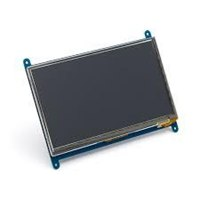
\includegraphics[width=\linewidth,height=0.18\textheight,keepaspectratio]{figures/ch10/touchscreen-mount}
    \caption{Touchscreen mounted on the wheelchair armrest.}
    \label{fig:touchscreen-mount}
\end{figure}
\begin{figure}[tbp]
    \centering
    \begin{subfigure}[t]{0.48\textwidth}
        \centering
        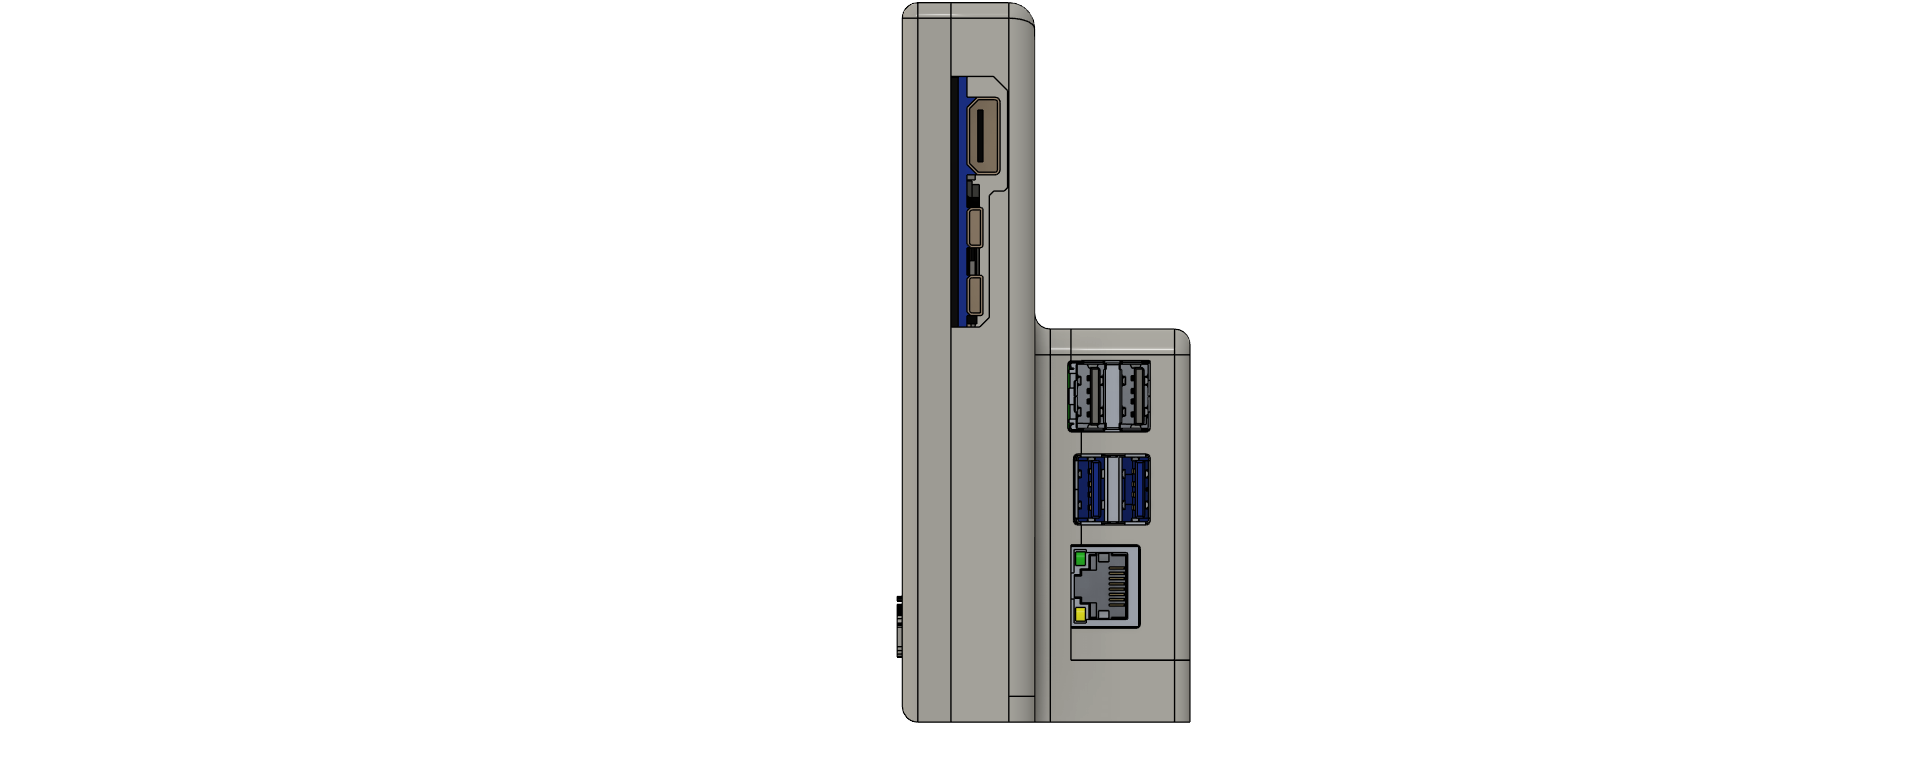
\includegraphics[width=\linewidth,height=0.20\textheight,keepaspectratio]{figures/ch10/touchscreen-holder-cad-folded}
        \caption{CAD, folded position.}
        \label{fig:touchscreen-holder-cad-folded}
    \end{subfigure}
    \hfill
    \begin{subfigure}[t]{0.48\textwidth}
        \centering
        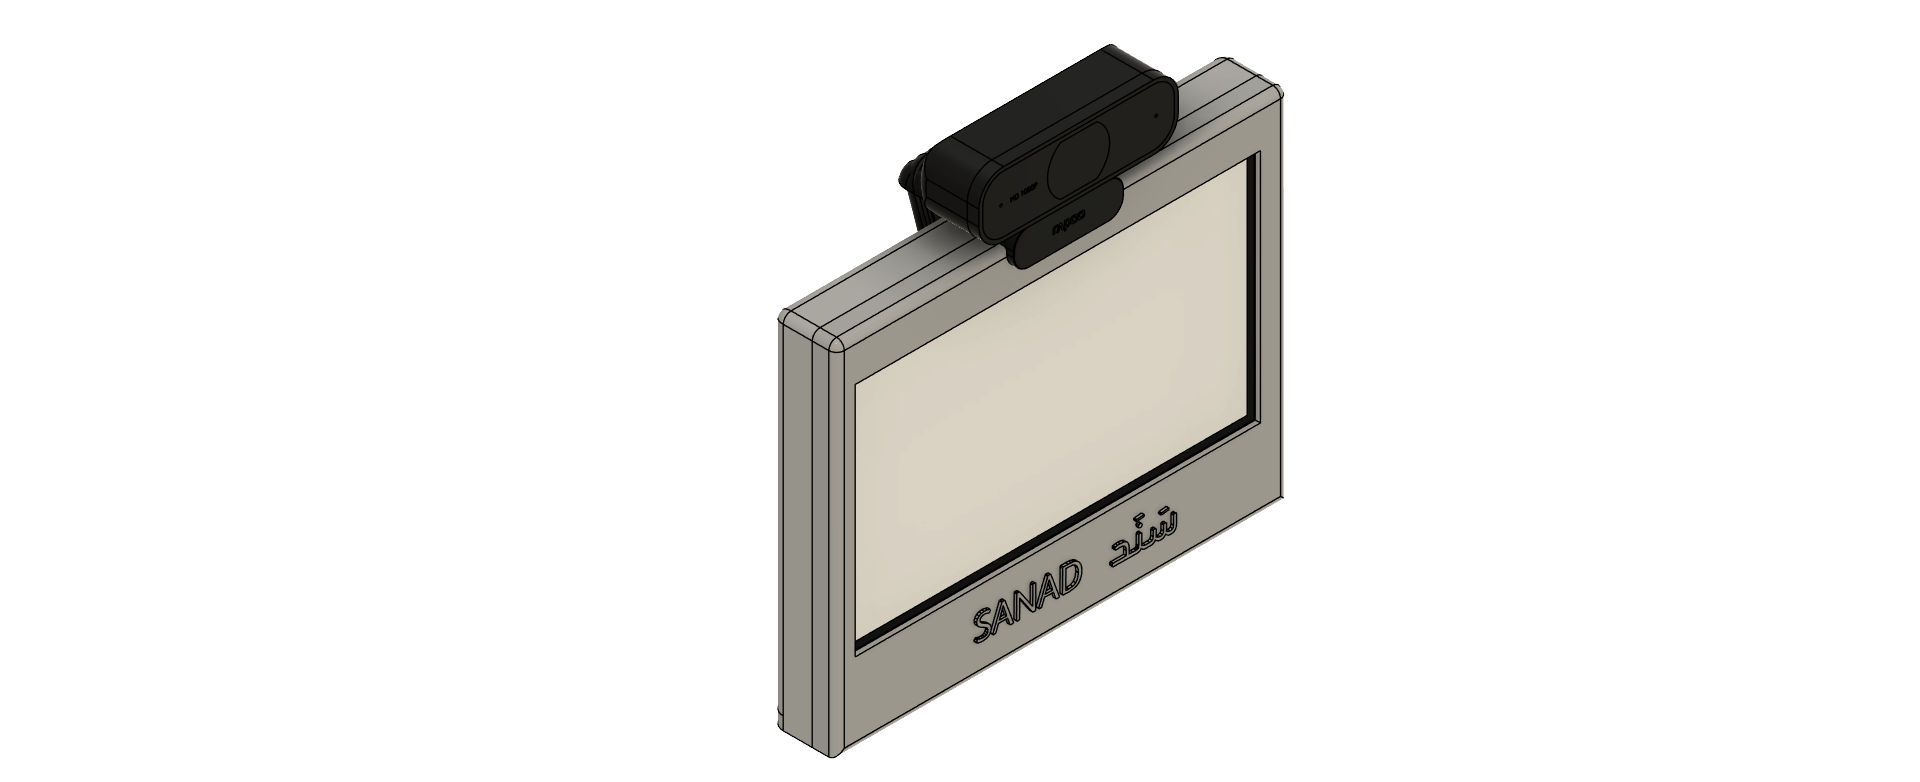
\includegraphics[width=\linewidth,height=0.20\textheight,keepaspectratio]{figures/ch10/touchscreen-holder-cad-unfolded}
        \caption{CAD, unfolded/deployed position.}
        \label{fig:touchscreen-holder-cad-unfolded}
    \end{subfigure}
    \medskip
    \begin{subfigure}[t]{0.48\textwidth}
        \centering
        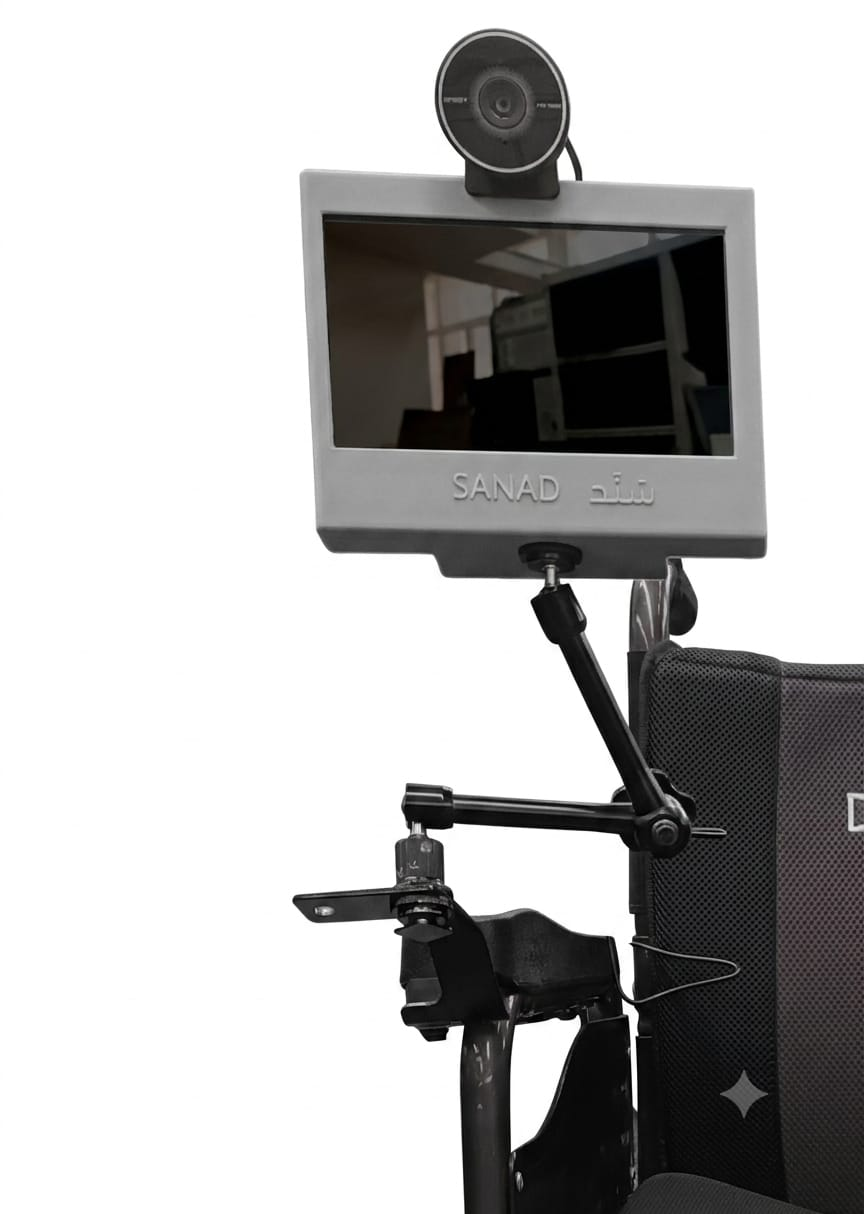
\includegraphics[width=\linewidth,height=0.20\textheight,keepaspectratio]{figures/ch10/:touchscreen-holder-real}
        \caption{Printed part on the armrest.}
        \label{fig:touchscreen-holder-real}
    \end{subfigure}
    \caption{Touchscreen holder: (a) CAD, folded position, (b) CAD, unfolded/deployed position, (c) printed part installed on the armrest.}
    \label{fig:touchscreen-holder}
\end{figure}
The hinge mechanism shown in Figures~\ref{fig:touchscreen-holder-cad-folded} and~\ref{fig:touchscreen-holder-cad-unfolded} lets the screen fold flat against the armrest for storage and swing up into its deployed position for use. Figure~\ref{fig:touchscreen-holder-real} shows the printed bracket installed and holding the screen in place.
\FloatBarrier

\subsection{Complete System Integration}

The complete integrated design was modeled in Autodesk Fusion before fabrication, allowing every sensor mount and cable route to be checked for interference prior to printing.

\begin{figure}[H]
    \centering
    \begin{subfigure}[t]{0.48\textwidth}
        \centering
        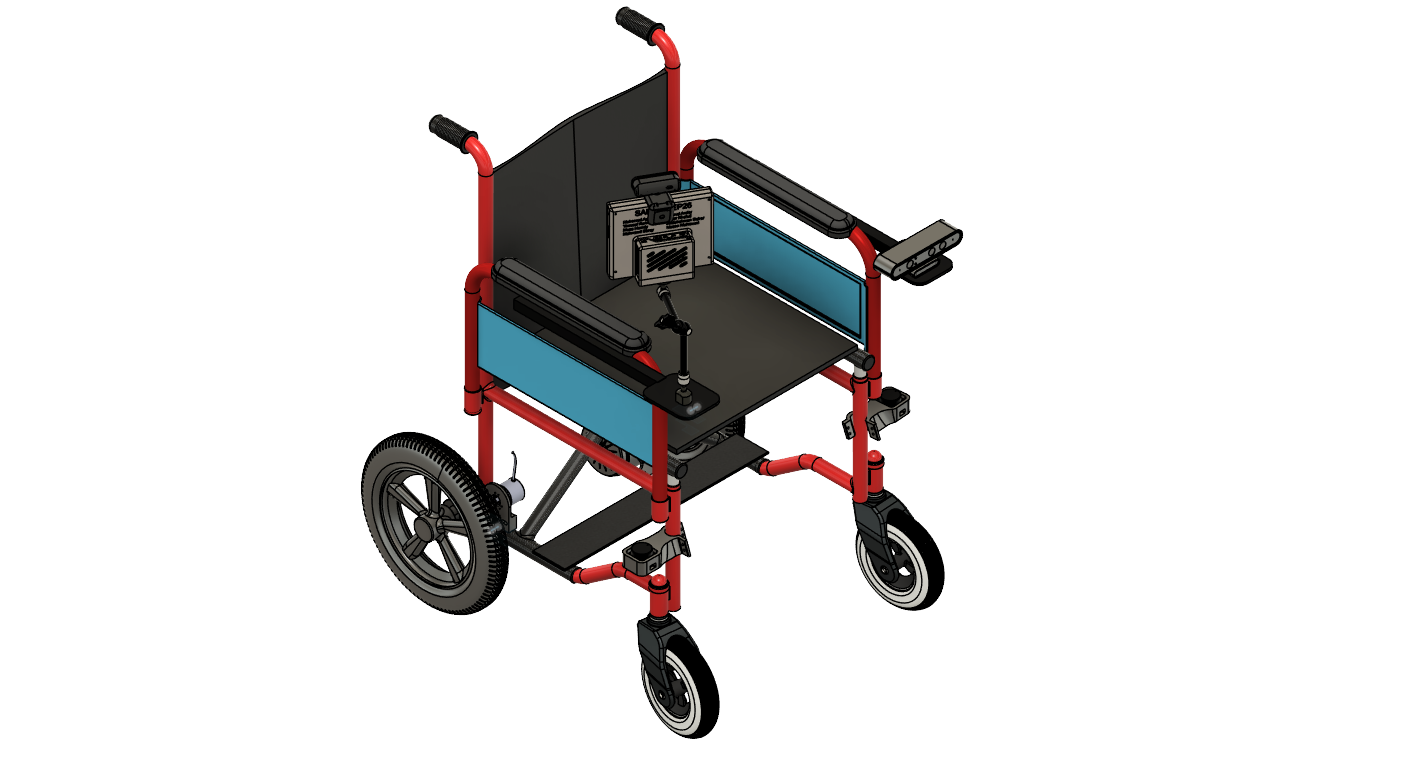
\includegraphics[height=0.28\textheight,keepaspectratio]{figures/ch10/full-wheelchair-cad-front}
        \caption{Front/isometric view.}
        \label{fig:full-wheelchair-cad-front}
    \end{subfigure}\hfill
    \begin{subfigure}[t]{0.48\textwidth}
        \centering
        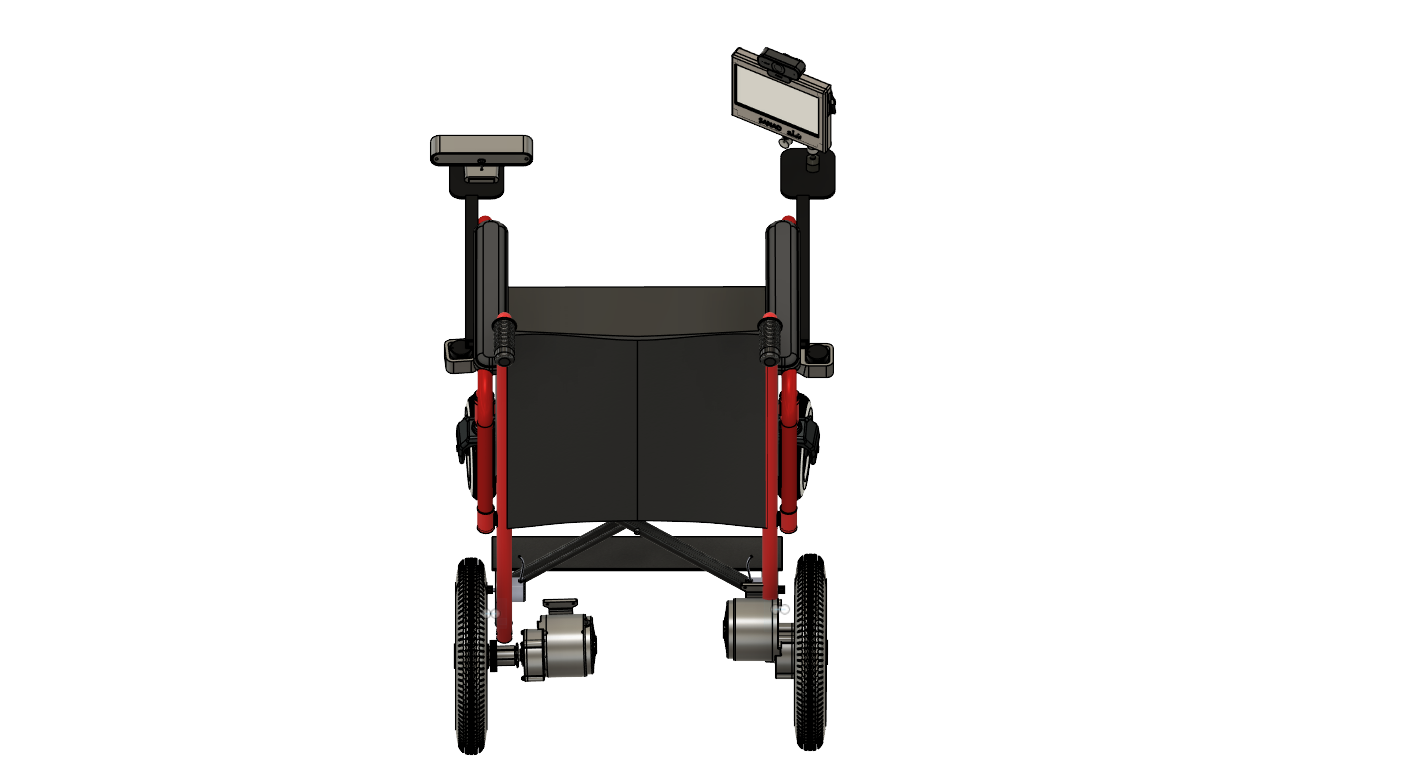
\includegraphics[height=0.28\textheight,keepaspectratio]{figures/ch10/full-wheelchair-cad-rear}
        \caption{Rear view.}
        \label{fig:full-wheelchair-cad-rear}
    \end{subfigure}
    \caption{Complete Sanad wheelchair -- CAD assembly: (a) front/isometric view, (b) rear view.}
    \label{fig:full-wheelchair-cad}
\end{figure}

Figure~\ref{fig:full-wheelchair-cad} shows the full CAD assembly with the dual LiDAR bar, depth camera, IMU, touchscreen, motor drivers, and rear-mounted encoders in their final relative positions.

\begin{figure}[H]
    \centering
    \begin{subfigure}[t]{0.48\textwidth}
        \centering
        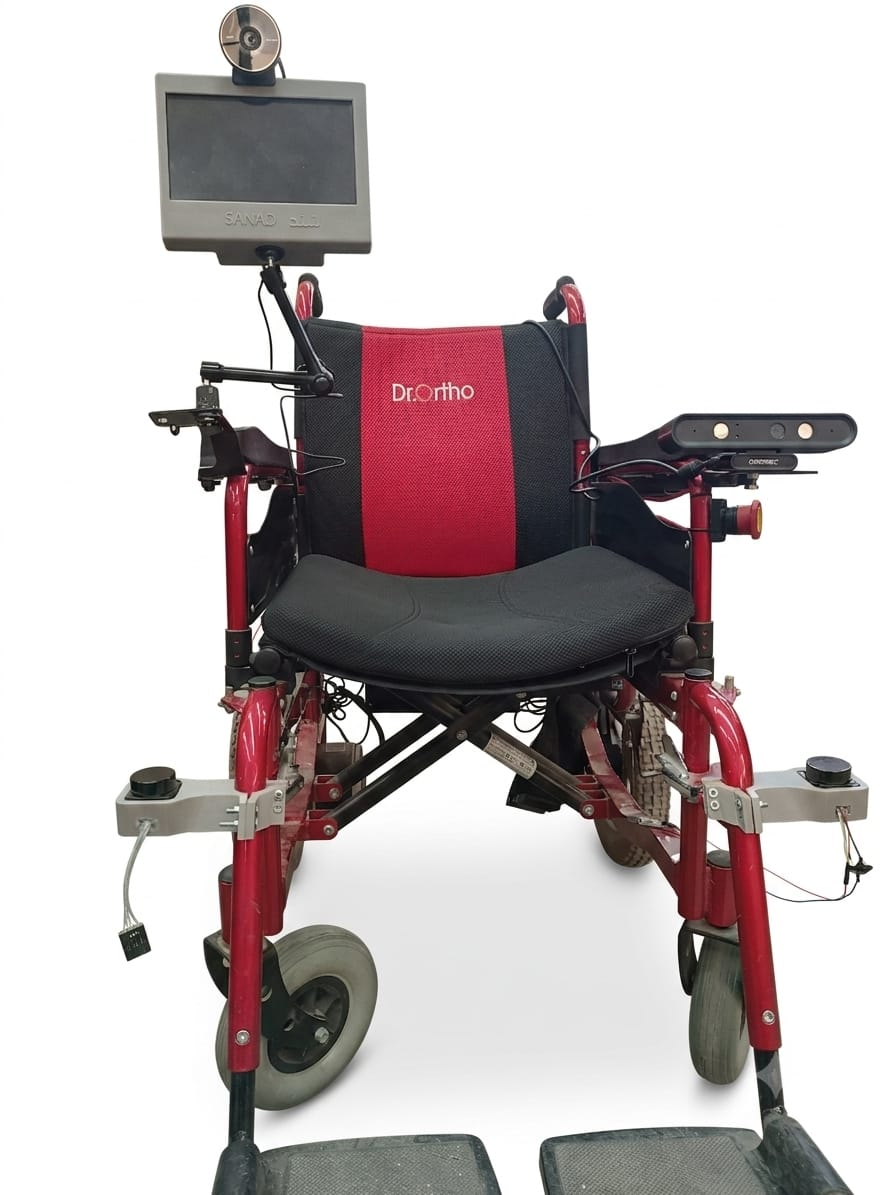
\includegraphics[height=0.28\textheight,keepaspectratio]{figures/ch10/full-wheelchair-real-front}
        \caption{Front view.}
        \label{fig:full-wheelchair-real-front}
    \end{subfigure}\hfill
    
    
    \label{fig:full-wheelchair-real}
\end{figure}

Figure~\ref{fig:full-wheelchair-real} shows the fully assembled wheelchair after all modules were installed, matching the CAD design shown above.

\section{Drivetrain Design Calculations}
This section presents the mechanical calculations used to verify that the drivetrain can safely carry the intended passenger load under normal operating conditions. The analysis is based on the rated motor power, wheel geometry, and rolling resistance, and is used to define a safe maximum payload for the wheelchair.

\subsection*{Design Data}

Table~\ref{tab:design-data} lists the key design parameters used in the calculations that follow.

\begin{table}[H]
\centering
\caption{The key design parameters used in the calculations are}
\label{tab:design-data}
\begin{tabular}{l c c c}
\hline
Parameter& Value  \\
\hline
Rated Power & 250W  \\
Maximum Speed & 8 km/h (2.22 m/s)\\
Wheel Radius &127 mm \\
Wheelchair Mass& 46 kg  \\
Rolling Resistance Coefficient & 0.06 \\
Factor of Safety & 1.2 \\
\hline
\end{tabular}
\end{table}


\subsection*{Assumptions}
The following simplifying assumptions were adopted to keep the analysis tractable while remaining representative of typical indoor operating conditions:
\begin{itemize}
\item Level ground.
\item Constant speed.
\item Rolling resistance only (aerodynamic drag and grade resistance neglected).
\item Rated power available at the wheels.
\end{itemize}

\subsection*{Calculations}
Using the design data in Table~\ref{tab:design-data} and the assumptions above, the wheel torque, tractive force, and maximum safe payload were calculated as follows.
\[
\omega = \frac{v}{r} = \frac{2.22}{0.127} = 17.5\ \mathrm{rad/s}
\]
\[
T = \frac{P}{\omega} = \frac{250}{17.5} = 14.3\ \mathrm{N\,m}
\]
\[
F = \frac{T}{r} = 112.6\ \mathrm{N}
\]
Rolling resistance force:
\[
F_{rr} = \mu (46 + m_{\text{load}}) g
\]
Setting the tractive force equal to the rolling resistance force and solving for the load mass gives a theoretical maximum passenger load of approximately 145.3\,kg. Applying the factor of safety of 1.2 gives the recommended design passenger load of approximately 121.1\,kg.

A factor of safety of 1.2 was selected because the wheelchair is intended for indoor operation on smooth, level floors under controlled loading conditions. This safety margin accounts for minor variations in rolling resistance, drivetrain efficiency, battery performance, and manufacturing tolerances while avoiding excessive oversizing.
\subsection*{Conclusion}
Based on the assumed operating conditions, the theoretical maximum passenger load is
approximately 145.3 kg. Applying a factor of safety of 1.2 gives a recommended design
passenger load of approximately 121 kg, which is consistent with the manufacturer's rated
capacity of 120 kg for the base wheelchair platform.

\subsection*{Motor Calculations}

The rated current of one DC motor is calculated from the rated power and supply voltage as

\[
I_{\text{rated}}=\frac{P}{V}
=\frac{250}{24}
=10.4~\mathrm{A}
\]

In practice, during normal indoor driving at moderate speeds, DC wheelchair motors typically draw only 20--50\% of their rated current. Therefore, the expected operating current of one motor is

\[
I_{\text{motor (normal)}} \approx 4\text{--}6~\mathrm{A}
\]

For two motors, the total operating current becomes

\[
I_{\text{total (normal)}} \approx 8\text{--}12~\mathrm{A}
\]

At startup, DC brushed motors typically draw approximately three times their rated current. Assuming a startup factor of 3,

\[
I_{\text{start}}
=3\times10.4
=31.2~\mathrm{A}
\]

The wheelchair uses two BTS7960 motor drivers, each capable of handling approximately \(43~\mathrm{A}\) peak current. Therefore,

\[
31.2~\mathrm{A}<43~\mathrm{A}
\]

which satisfies the current handling capability of the motor driver.    
\section{Motor Control \& PID Tuning}
The wheelchair utilizes two BTS7960 high-current motor drivers controlled by an Arduino Nano microcontroller to regulate the speed and direction of the two drive motors. Wheel velocity feedback is obtained from the wheel encoders, enabling the implementation of a closed-loop speed control system based on a PID controller.
\subsection*{Control Loop}
Figure~\ref{fig:control-loop} illustrates the complete end-to-end motor control loop, starting from the \texttt{cmd\_vel} velocity command generated by the navigation stack, through the PID controller and motor driver, to the DC motor. Encoder feedback is continuously returned to the controller, forming a closed-loop control system that ensures accurate speed regulation and reliable motor performance.

\begin{figure}[H]
\centering
\begin{tikzpicture}[>=stealth, node distance=10mm, every node/.style={font=\small}]
\tikzstyle{block}=[draw, rounded corners, minimum width=3cm, minimum height=8mm, align=center]
\node[block] (cmdvel) {cmd\_vel};
\node[block, below=of cmdvel] (rpi) {Raspberry Pi 5};
\node[block, below=of rpi] (nano) {Arduino Nano};
\node[block, below=of nano] (pid) {PID Controller};
\node[block, below=of pid] (driver) {BTS7960 Driver};
\node[block, below=of driver] (motor) {Motor};
\node[block, below=of motor] (encoder) {Encoder Feedback};

\draw[->] (cmdvel) -- (rpi);
\draw[->] (rpi) -- node[left, font=\scriptsize]{UART} (nano);
\draw[->] (nano) -- (pid);
\draw[->] (pid) -- node[left, font=\scriptsize]{PWM} (driver);
\draw[->] (driver) -- (motor);
\draw[->] (motor) -- (encoder);
\draw[->] (encoder.west) -| ++(-1.4,0) |- (pid.west);
\end{tikzpicture}
\caption{End-to-end motor control loop from cmd\_vel to encoder feedback.}
\label{fig:control-loop}
\end{figure}
The Raspberry Pi 5 generates the desired wheel velocities through the \texttt{cmd\_vel} command and transmits them to the Arduino Nano via serial (UART) communication. The Arduino compares the desired velocity with the actual wheel speed measured by the encoders and computes the control signal using the PID algorithm. The resulting PWM signal is then sent to the BTS7960 motor driver to regulate the motor speed.


\subsection*{PID Structure}
The Arduino Nano implements a discrete PID controller for each wheel that converts the velocity error into a PWM duty-cycle command. Figure~\ref{fig:pid-structure} shows the general structure of this control loop. The PID controller output is:
\[
u(t) = K_p e(t) + K_i \int e(t)\,dt + K_d \frac{d e(t)}{dt}
\]
where
\[
e(t) = \text{setpoint} - \text{measured value}.
\]

Proportional control reacts to the current error. Increasing $K_p$ generally produces a faster response and smaller error, while too large a value can cause oscillation. Integral control accumulates past errors, removing steady-state error and helping the motor reach the target RPM; however, too much integral gain can lead to overshoot and oscillation. Derivative control predicts future behavior based on the error rate of change, reducing overshoot and improving stability.

\begin{figure}[H]
\centering
\begin{tikzpicture}[>=stealth,node distance=20mm,every node/.style={font=\footnotesize}]
\tikzstyle{block}=[draw,fill=gray!20,rounded corners,minimum width=2.6cm,minimum height=1cm,align=center]
\tikzstyle{sum}=[draw,circle,fill=gray!10,minimum size=9mm,inner sep=0pt]

\node[sum] (sum) {};
\node[left=8mm of sum] (ref) {Reference};
\node[above left=1mm and .5mm of sum,font=\scriptsize] {$+$};
\node[below left=1mm and .5mm of sum,font=\scriptsize] {$-$};

\node[block,right=20mm of sum] (pid) {Controller\\PID};
\node[block,right=22mm of pid] (plant) {Plant\\(Motor, etc.)};

\draw[->] (ref) -- (sum);
\draw[->] (sum) -- node[midway,above=3mm]{Error} (pid);
\draw[->] (pid) -- node[midway,above=3mm]{PWM Value} (plant);
\draw[->] (plant.east) -- ++(25mm,0);

\coordinate (corner) at ($(plant.south)+(0,-8mm)$);
\coordinate (fb) at ($(sum.south |- corner)$);

\draw (plant.south) -- (corner);
\draw (corner) -- node[midway,below=4mm]{Encoder} (fb);
\draw[->,shorten >=2pt] (fb) -- node[midway,left=6mm]{Actual value} (sum.south);

\end{tikzpicture}
\caption{General PID control loop structure used for wheel speed control.}
\label{fig:pid-structure}
\end{figure}
\subsection*{The PID controller output is:}
\[
u(t)=K_p\,e(t)+K_i\int_{0}^{t}e(\tau)\,d\tau+K_d\frac{de(t)}{dt}
\]
\subsection*{Where:}
\begin{itemize}
    \item P = Proportional term
    \item I = Integral term
    \item  D = Derivative term
    \item  e(t): Control error, defined as:
     e(t) = setpoint − measured value
\end{itemize}

\begin{enumerate}
    \item \textbf{Proportional Control (P)} \\
   \\ The proportional term reacts to the current error.\\
   \textbf{Effect of increasing Kp:} 
   \begin{itemize}
       \item Faster response.
       \item Smaller steady-state error.
       \item Too large → oscillation
   \end{itemize}

Figure~\ref{fig:kp-effect} illustrates the effect of increasing $K_p$ on the speed response.

\begin{figure}[H]
\centering
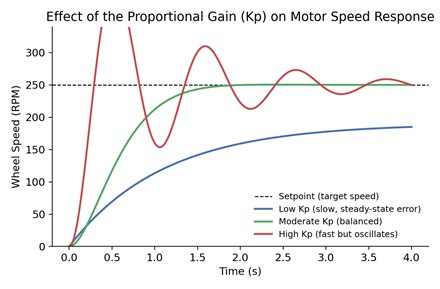
\includegraphics[width=0.5\linewidth,keepaspectratio]{figures/ch10/kp-effect}
\caption{Illustrative effect of increasing proportional gain on the speed response.}
\label{fig:kp-effect}
\end{figure}

\item \textbf{Integral Control (I)} \\
    \\The integral term accumulates and remembers past errors.
    \\  \textbf{Effect of increasing KI:} 
     \begin{itemize}
       \item Removes steady-state error.
       \item Helps the motor reach exactly the target RPM.
       \item Too high → overshoot and oscillation.
   \end{itemize}

Figure~\ref{fig:ki-effect} illustrates the effect of increasing $K_i$ on the steady-state error.

\begin{figure}[H]
\centering
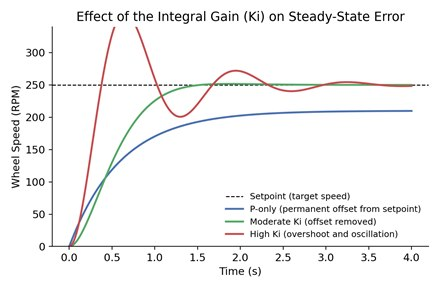
\includegraphics[width=0.5\linewidth,keepaspectratio]{figures/ch10/ki-effect}
\caption{Illustrative effect of integral gain on steady-state error.}
\label{fig:ki-effect}
\end{figure}
 \item \textbf{Derivative Control (D)} \\
    \\The derivative term predicts future behavior by looking at how fast the error changes.
    \\  \textbf{Effect of increasing Kd:} 
     \begin{itemize}
       \item Reduces overshoot.
       \item Improves stability.
   \end{itemize}
     \end{enumerate}

Figure~\ref{fig:kd-effect} illustrates the effect of increasing $K_d$ on overshoot and stability.

\begin{figure}[H]
\centering
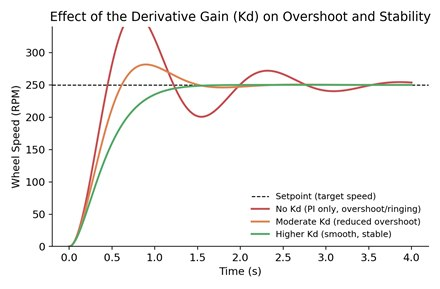
\includegraphics[width=0.5\linewidth,keepaspectratio]{figures/ch10/kd-effect}
\caption{Illustrative effect of derivative gain on overshoot and stability.}
\label{fig:kd-effect}
\end{figure}

% ============================================================
% EDIT: The Ziegler--Nichols tuning subsection below has been commented out
% and replaced with a trial-and-error tuning subsection, per user request.
% ============================================================
% \subsection*{PID Tuning Using the Ziegler--Nichols Method}
% The PID controller parameters were initially tuned using the Ziegler--Nichols closed-loop tuning method, which provides a systematic approach for estimating controller gains.
%
% The tuning procedure consists of the following steps:
% \begin{enumerate}
% \item Set the integral and derivative gains to zero: $K_i = 0$, $K_d = 0$.
% \item Gradually increase the proportional gain $K_p$ until the motor output exhibits continuous and stable oscillations.
% \item Record the proportional gain at which sustained oscillation occurs. This value is known as the Ultimate Gain ($K_u$).
% \item Measure the oscillation period, known as the Ultimate Period ($P_u$).
% \item Compute the PID parameters using the Ziegler--Nichols tuning rules:
% \end{enumerate}
% \begin{itemize}
%     \item $K_p = 0.6 K_u$, 
%     \item $K_i = 2 K_p / P_u$,
%     \item $K_d = K_p P_u / 8$.
%
% \end{itemize}
%
% \subsection*{Advantages of using Ziegler–Nichols tuning}
% \begin{itemize}
%     \item Provides a systematic and repeatable tuning procedure.
%     \item Produces reasonable initial gain values without requiring an accurate mathematical
% model
%     \item Reduces manual trial-and-error tuning efforts.
%     \item Enables rapid deployment of the motor control system.
%     \item Serves as an effective starting point for further experimental optimization.
% \end{itemize}

\subsection*{PID Tuning Using a Trial-and-Error Method}
The PID controller parameters were tuned experimentally using a manual trial-and-error approach.

The tuning procedure consists of the following steps:
\begin{enumerate}
\item Start with only the proportional gain enabled ($K_i = 0$, $K_d = 0$) and gradually increase $K_p$ while observing the wheel speed response, until a reasonable trade-off is reached between fast response and acceptable oscillation.
\item Introduce a small integral gain $K_i$ and increase it gradually to eliminate steady-state error, so the motor reliably reaches the target RPM.
\item Add a small derivative gain $K_d$ and increase it gradually to damp any remaining oscillation and improve overall stability.
\item Repeat the above steps under different payload conditions to confirm the selected gains remain acceptable across the expected range of user weights.
\end{enumerate}

\subsection*{Advantages of the trial-and-error tuning approach}
\begin{itemize}
    \item Does not require an accurate mathematical model of the motor--wheelchair system.
    \item Allows the gains to be adjusted directly based on the observed real-world response, including nonlinearities that an analytical model would not capture.
    \item Simple to apply with basic test equipment and no specialized instrumentation.
    \item Well suited to iterative refinement of the gains across different payloads and operating conditions.
\end{itemize}





\section{Hardware Circuit \& Power System}
This section describes the electrical implementation of the wheelchair, covering both the custom motor-control interface circuit and the overall power distribution architecture. Together, these subsystems ensure that every sensor, actuator, and compute module receives clean, adequately rated power while keeping wiring between the Arduino Nano, the motor drivers, and the encoders as short and reliable as possible.

\subsection{Motor Control \& Encoder Interface Board}

A custom interface board was developed around the Arduino Nano to simplify the electrical connections between the microcontroller, the two BTS7960 motor drivers, and the dual quadrature wheel encoders. Instead of wiring each module individually, the board integrates all signal and power connections into a compact PCB with clearly labeled connectors.

The interface board includes a dedicated terminal Block power input, separate connectors for the left and right motor drivers, and dedicated headers for both wheel encoders. This arrangement minimizes wiring complexity, improves assembly reliability, simplifies maintenance, and reduces the likelihood of connection errors. The compact design also allows the complete motor control electronics to be mounted beneath the wheelchair seat alongside the motor drivers.

% TODO (pending clarification): user asked to enlarge subfigure (b) of "figure 10.99"
% so it is readable. The most likely candidate in this chapter is the electrical
% schematic below (subfigure (b) of the PCB figure), since schematics tend to have
% small text/labels, but this has NOT been resized yet -- waiting to confirm which
% figure was meant before changing its size.
Figure~\ref{fig:PCB} presents the custom interface board. The PCB layout is shown in Figure~\ref{fig:PCB}(a), while the corresponding electrical schematic is shown in Figure~\ref{fig:PCB}(b).

\begin{figure}[H]
\centering

\begin{figure}[H]
\centering
\begin{subfigure}[t]{0.55\textwidth}
    \centering
    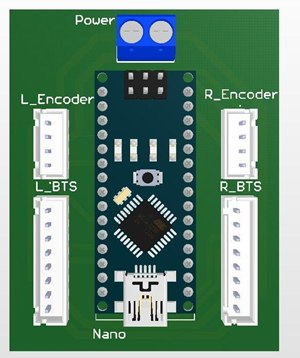
\includegraphics[width=0.8\linewidth]{figures/ch10/PCB}
    \caption{Custom PCB layout.}
\end{subfigure}

\vspace{0.3cm}

\begin{subfigure}[t]{0.9\textwidth}
    \centering
    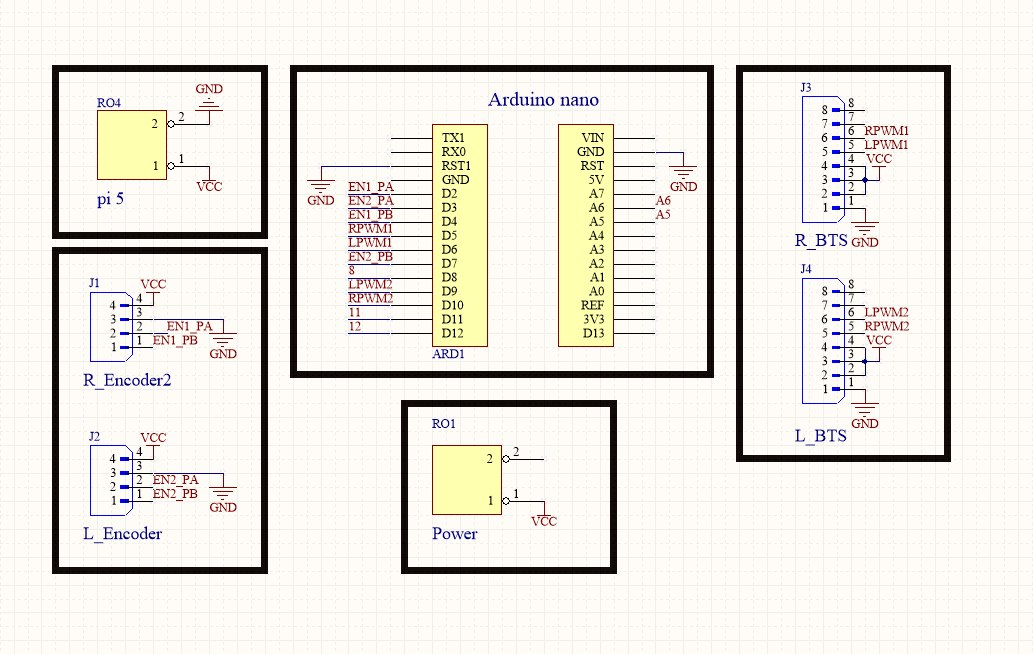
\includegraphics[width=0.85\linewidth]{figures/ch10/PCB_Schematic}
    \caption{Electrical schematic of the interface board.}
\end{subfigure}

\caption{Arduino Nano motor control and encoder interface board: (a) custom PCB layout and (b) electrical schematic.}
\label{fig:PCB}
\end{figure}
  
  \caption{Arduino Nano motor control and encoder interface board: (a) custom PCB layout and (b) electrical schematic.}
  \label{fig:PCB}
\end{figure}
\caption{Arduino Nano motor control and encoder interface board: (a) custom PCB layout and (b) electrical schematic.}
\label{fig:PCB}
\end{figure}
\subsection{Power Distribution Architecture}
Electrical power for the compute and sensing subsystems is supplied by a dedicated 12V,
23.45Ah lithium-ion battery, separate from the wheelchair's original 24V drive battery. A voltage
sensor continuously monitors this battery for health and charge-state monitoring. An inline fuse
is placed immediately after the battery's positive terminal, ahead of the branch to the voltage
sensor and the two buck converters, to protect the battery, wiring, and downstream electronics
against short-circuit and overcurrent conditions. Two buck
converters step the 12V supply down to a regulated 5V rail: a 7A converter dedicated to the
Raspberry Pi 5 main compute unit, and a 12A converter that supplies all remaining peripherals.
The 12A rail is distributed through internal USB connections to the dual LiDAR units, the depth
camera, and the Arduino Nano, through external USB connections to the head-mounted IMU, the
IR module, the hand biometric sensor, and the microphone, and through dedicated USB femaleterminals to the secondary Raspberry Pi 4 (which drives the touchscreen and eye-tracking
interface), the 7-inch screen, and the speaker output. Figure~\ref{fig:power-distribution} illustrates the complete power
distribution tree, including the protective fuse placed between the battery and the downstream loads.

\begin{figure}[H]
\centering
\resizebox{\textwidth}{!}{%
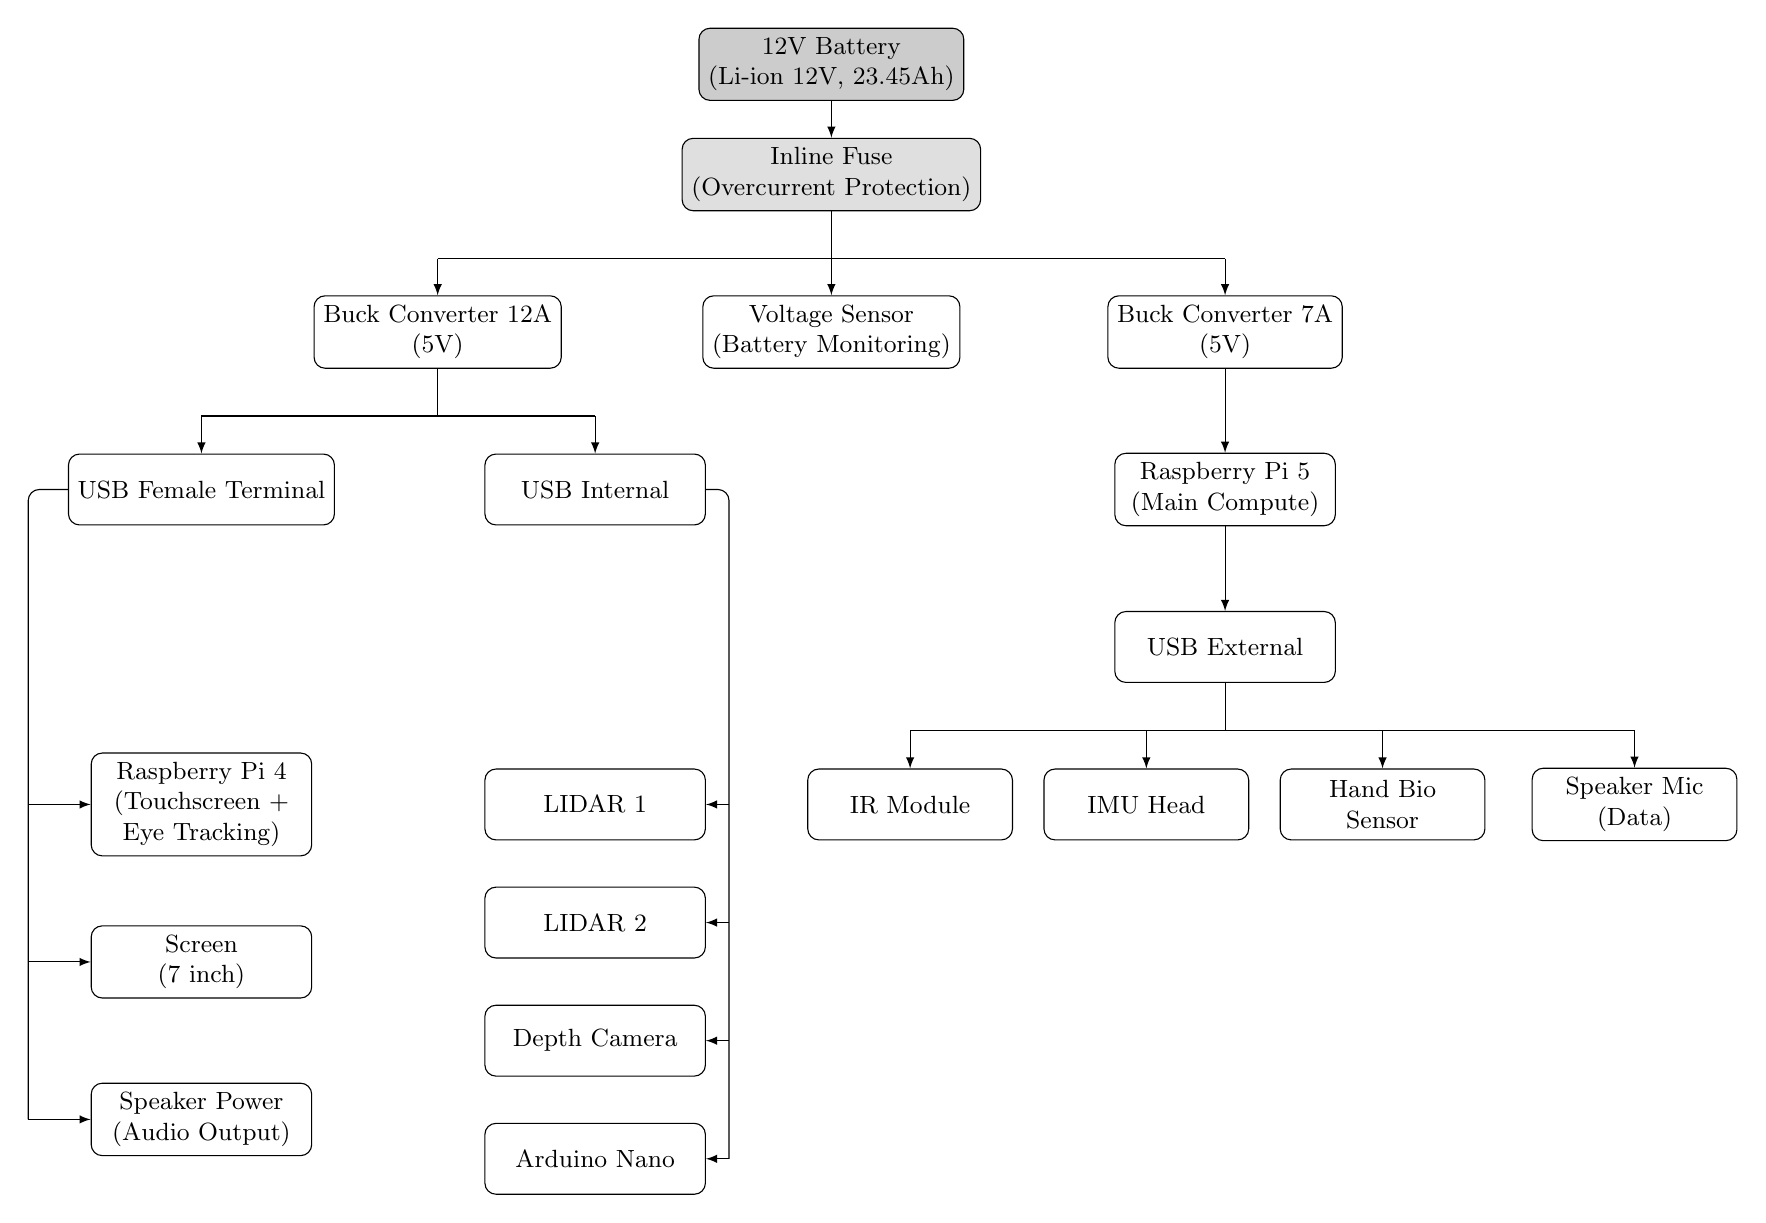
\begin{tikzpicture}[
>=latex,
node distance=1.1cm,
block/.style={
draw,
rounded corners,
minimum width=2.8cm,
minimum height=0.9cm,
align=center,
font=\small
},
bus/.style={
draw,
rounded corners,
minimum width=3.2cm,
minimum height=0.9cm,
align=center,
font=\small
},
every path/.style={rounded corners}
]
%========================
% Top Level
%========================
\node[block,fill=gray!40] (battery)
{12V Battery\\(Li-ion 12V, 23.45Ah)};
\node[block,fill=gray!25] (fuse) at (0,-1.4)
{Inline Fuse\\(Overcurrent Protection)};
\node[block] (buck12) at (-5,-3.4)
{Buck Converter 12A\\(5V)};
\node[block] (sensor) at (0,-3.4)
{Voltage Sensor\\(Battery Monitoring)};
\node[block] (buck7) at (5,-3.4)
{Buck Converter 7A\\(5V)};
% ---- Battery: through the fuse, ONE trunk out, then branch to 3 ----
\draw[->] (battery.south) -- (fuse.north);
\draw (fuse.south) -- ++(0,-0.6) coordinate (battrunk);
\draw (battrunk -| buck12.north) -- (battrunk -| buck7.north);
\draw[->] (battrunk -| buck12.north) -- (buck12.north);
\draw[->] (battrunk)                -- (sensor.north);
\draw[->] (battrunk -| buck7.north) -- (buck7.north);
%========================
% Left Side
%========================
\node[block] (usbf) at (-8,-5.4)
{USB Female Terminal};
\node[block] (usbi) at (-3,-5.4)
{USB Internal};
% ---- buck12: ONE trunk out, then branch to 2 ----
\draw (buck12.south) -- ++(0,-0.6) coordinate (b12trunk);
\draw (b12trunk -| usbf.north) -- (b12trunk -| usbi.north);
\draw[->] (b12trunk -| usbf.north) -- (usbf.north);
\draw[->] (b12trunk -| usbi.north) -- (usbi.north);
% ---- USB Female Terminal: turn 90 right beside block, then straight down till last block ----
\node[block] (rpi4) at (-8,-9.4)
{Raspberry Pi 4\\(Touchscreen +\\Eye Tracking)};
\node[block] (screen) at (-8,-11.4)
{Screen\\(7 inch)};
\node[block] (speaker) at (-8,-13.4)
{Speaker Power\\(Audio Output)};
\draw (usbf.west) -| (-10.2,-13.4);
\draw[->] (-10.2,-9.4)  -- (rpi4.west);
\draw[->] (-10.2,-11.4) -- (screen.west);
\draw[->] (-10.2,-13.4) -- (speaker.west);
% ---- USB Internal: turn 90 right beside block, then straight down till last block ----
\node[block] (lidar1) at (-3,-9.4)
{LIDAR 1};
\node[block] (lidar2) at (-3,-10.9)
{LIDAR 2};
\node[block] (depth) at (-3,-12.4)
{Depth Camera};
\node[block] (nano) at (-3,-13.9)
{Arduino Nano};
\draw (usbi.east) -| (-1.3,-13.9);
\draw[->] (-1.3,-9.4)    -- (lidar1.east);
\draw[->] (-1.3,-10.9)  -- (lidar2.east);
\draw[->] (-1.3,-12.4)   -- (depth.east);
\draw[->] (-1.3,-13.9) -- (nano.east);
%========================
% Right Side
%========================
\node[block] (rpi5) at (5,-5.4)
{Raspberry Pi 5\\(Main Compute)};
\node[block] (usbext) at (5,-7.4)
{USB External};
\draw[->] (buck7.south) -- (rpi5.north);
\draw[->] (rpi5.south) -- (usbext.north);
%========================
% External devices
%========================
\node[
draw,
rounded corners,
minimum width=2.6cm,
minimum height=0.9cm,
font=\small,
align=center
] (ir) at (1,-9.4)
{IR Module};
\node[
draw,
rounded corners,
minimum width=2.6cm,
minimum height=0.9cm,
font=\small,
align=center
] (imu) at (4,-9.4)
{IMU Head};
\node[
draw,
rounded corners,
minimum width=2.6cm,
minimum height=0.9cm,
font=\small,
align=center
] (bio) at (7,-9.4)
{Hand Bio\\Sensor};
\node[
draw,
rounded corners,
minimum width=2.6cm,
minimum height=0.9cm,
font=\small,
align=center
] (mic) at (10.2,-9.4)
{Speaker Mic\\(Data)};
% ---- USB External: ONE trunk out, then branch to 4 ----
\draw (usbext.south) -- ++(0,-0.6) coordinate (uexttrunk);
\draw (uexttrunk -| ir.north) -- (uexttrunk -| mic.north);
\draw[->] (uexttrunk -| ir.north)  -- (ir.north);
\draw[->] (uexttrunk -| imu.north) -- (imu.north);
\draw[->] (uexttrunk -| bio.north) -- (bio.north);
\draw[->] (uexttrunk -| mic.north) -- (mic.north);
\end{tikzpicture}
}
\caption{Power distribution architecture, including the protective inline fuse placed between the battery and the downstream regulation stages.}
\label{fig:power-distribution}
\end{figure}
\subsection{Power Consumption Analysis}
To size the buck converters and estimate battery runtime, the maximum power consumption of each component was tabulated for both 5\,V rails. Table~\ref{tab:power-rpi5-rail} lists the components on the 7~A Raspberry Pi 5 rail, Table~\ref{tab:power-12a} lists the components on the 12~A peripheral rail, and Table~\ref{tab:power-summary} summarizes the totals for both rails.

\begin{table}[H]
\centering
\caption{Raspberry Pi 5 rail power consumption.}
\label{tab:power-rpi5-rail}
\begin{tabular}{l c c c}
\hline
Component & Voltage (V) & Max Current (A) & Power (W) \\
\hline
IMU Head Sensor & 5 & 0.05 & 0.25 \\
IR Module & 5 & 0.03 & 0.15 \\
Hand Bio Sensor & 5 & 0.10 & 0.50 \\
USB Microphone & 5 & 0.10 & 0.50 \\
\hline
Total & -- & 0.28 & 1.40 \\
\hline
\end{tabular}
\end{table}

\begin{table}[H]
\centering
\caption{Buck converter 12\,A (5\,V) rail power consumption.}
\label{tab:power-12a}
\begin{tabular}{l c c c}
\hline
Component & Voltage (V) & Max Current (A) & Power (W) \\
\hline
Raspberry Pi 4 & 5 & 2.5 & 12.5 \\
Screen (7 inch) & 5 & 0.74 & 3.7 \\
Speaker Power & 5 & 1.00 & 5.0 \\
LiDAR (LD06) -- unit 1 & 5 & 0.30 & 1.5 \\
LiDAR (LD06) -- unit 2 & 5 & 0.30 & 1.5 \\
Depth Camera & 5 & 0.50 & 2.5 \\
Arduino Nano & 5 & 0.035 & 0.175 \\
\hline
Total & -- & 5.375 & 26.875 \\
\hline
\end{tabular}
\end{table}

\begin{table}[H]
\centering
\caption{Overall 5\,V rail power summary.}
\label{tab:power-summary}
\begin{tabular}{l c c}
\hline
Rail & Current (A) & Power (W) \\
\hline
Buck Converter 7\,A (5\,V) & 5 & 25 \\
Buck Converter 12\,A (5\,V) & 5.375 & 26.875 \\
\hline
Total & 10.375 & 51.875 \\
\hline
\end{tabular}
\end{table}

As summarized in Table~\ref{tab:power-summary}, the combined current draw on the 12\,V input battery is therefore approximately 10.375\,A, corresponding to a total power consumption of about 51.875\,W across both 5\,V rails. To protect the battery and wiring from fault conditions, an inline fuse rated above this normal operating current (e.g., a 15~A fuse, chosen to sit safely above the 10.375~A steady-state draw while still tripping well below typical wiring and connector current limits) is installed directly at the battery output, ahead of the voltage sensor and both buck converters, as shown in Figure~\ref{fig:power-distribution}.

\subsection*{Battery \& Runtime Estimation}
With the total power consumption established, the usable runtime of the 12\,V compute-and-sensor battery can be estimated from its rated energy capacity.
\[
\text{Battery Energy} = 12\ \text{V} \times 23.45\ \text{Ah} = 281.4\ \text{Wh}
\]
\[
\text{Estimated Runtime} = \frac{281.4\ \text{Wh}}{51.875\ \text{W}} \approx 5.42\ \text{h}
\]
This gives an estimated continuous runtime of approximately 5.4 hours for the compute and sensor subsystem under maximum load, which is independent of the wheelchair's separate 24\,V drive battery.

% ============================================================
\section{Bill of Materials \& Cost Estimation}
% ============================================================

To evaluate the economic feasibility of the Sanad autonomous wheelchair, a detailed Bill of Materials (BOM) has been compiled. One of the core design goals of Sanad was to construct a highly capable, autonomous cyber-physical platform using consumer-grade sensors and open-source software, keeping the total cost at a fraction of commercial smart wheelchairs, which often exceed \$10\,000 to \$20\,000 USD.

The hardware implementation is built upon a standard commercial powered wheelchair, retrofitted with sensors, an onboard host computer, low-level microcontrollers, and custom-designed 3D-printed mounts. Table~\ref{table:bom_cost_estimation} outlines the cost breakdown of the prototype in both Egyptian Pounds (EGP) and US Dollars (USD), based on market prices at the time of development.
\begin{table}[H]
\centering
\caption{Bill of Materials (BOM) and Cost Estimation for the Sanad Prototype.}
\label{table:bom_cost_estimation}
\small
\begin{tabularx}{\textwidth}{|l|X|c|r|r|}
\hline
\textbf{Category} & \textbf{Component Description} & \textbf{Qty} & \textbf{Unit Cost (EGP)} & \textbf{Total Cost (EGP)} \\
\hline
Chassis & Base Foldable Electric Wheelchair (24V, 250W motors) & 1 & 20,000 & 20,000 \\
\hline
Compute & Raspberry Pi 5 (8GB RAM) --- main compute & 1 & 14,000 & 14,000 \\
\hline
\multirow{3}{*}{Perception}
 & LD19 Planar LiDAR Rangefinder & 2 & 4,500 & 9,000 \\
\cline{2-5}
 & Front-Facing RGB-D Depth Camera & 1 & 7,500 & 7,500 \\
\cline{2-5}
 & BNO055 Inertial Measurement Unit (IMU) & 1 & 3,500 & 3,500 \\
\hline
Power & 12V 23.45Ah Battery Pack & 1 & 3,750 & 3,750 \\
\hline
Mechanical & 3D-Printed PETG Mounts, GT2 Pulley-Belt \& Fasteners & 1 & 2,000 & 2,000 \\
\hline
Electronics & Custom Arduino Nano Interface PCB + Dual Buck Converters (7A/12A) + Dual hub & 1 & 1,750 & 1,750 \\
\hline
\multicolumn{3}{|r|}{\textbf{Subtotal --- Base Platform (without Modules)}} & & \textbf{61,500 EGP} \\
\hline
\multirow{2}{*}{Modules}
 & Touchscreen Interface --- 7" LCD + Secondary Raspberry Pi 4 (8GB) & 1 & 3,000 + 9,400 & 12,400 \\
\cline{2-5}
 & Head-Motion Control --- Wearable IMU + ESP32-C3 & 1 & 950 + 250 & 1,200 \\
\hline
\multicolumn{3}{|l|}{\textbf{Total Project Cost (with Modules)}} & & \textbf{75,075 EGP} \\
\hline
\end{tabularx}
\end{table}

This estimation demonstrates that the entire autonomous and multi-modal platform can be assembled for approximately 75,075 EGP, including the touchscreen and head-motion assistive module stack. The base navigation-and-mobility platform alone — chassis, compute, perception, power, and control electronics, without either assistive module — costs approximately 61,500 EGP, meaning the two plug-and-play modules add roughly 13,575 EGP to the total. By leveraging open-source middleware (ROS 2, Nav2, SLAM Toolbox) and custom software logic, Sanad eliminates the prohibitive licensing fees associated with proprietary assistive technology, making autonomous mobility and smart home control accessible to middle- and lower-income families.

\section{Summary and Transition}
This chapter has detailed the physical design, fabrication choices, motor control tuning, and cost estimates of the Sanad wheelchair. The next chapter, Chapter 11 (Conclusion), concludes the book by synthesizing project achievements and outlining future design roadmaps.